\documentclass[orivec]{llncs}
\usepackage{graphicx}
\usepackage{amsmath}			% for "cases"
\usepackage{amsfonts}		% for frakur fonts
% \usepackage{mathrsfs}		% for curly "E" error symbol
\usepackage{float}
\usepackage[most]{tcolorbox}		% for wrapping example in color box
%\usepackage{wrapfig}		% wrap figure beside text, used in example
\usepackage{tikz-cd}			% commutative diagrams
\usepackage{tikz}
\usepackage{amssymb}			% for \multimap \updownarrow \bigstar \varnothing
\usepackage{sectsty}			% change section color
\usepackage[normalem]{ulem}	% underline with line breaks: /uline
%\usepackage{turnstile}		% longer turnstiles
\usepackage{wasysym}			% smileys
%\usepackage{cancel}			% center "not" line for "broken heart"
\usepackage{hyperref}		% refs, links become clickable
\usepackage[boxed]{algorithm2e}	% algorithms

% *************** Delete when not using Chinese or colors **********************
\usepackage{xeCJK}
\setCJKmainfont[BoldFont=SimHei,ItalicFont=KaiTi]{SimSun}
\usepackage{color}
\definecolor{Cerulean}{RGB}{100,100,200}
\newcommand{\emp}[1]{\textbf{\textcolor{Cerulean}{#1}}}
\definecolor{grey}{rgb}{0.9,0.9,0.9}  % grey

% \chapterfont{\color{blue}}  % sets colour of chapters
\sectionfont{\color{blue}} 
\subsectionfont{\color{blue}} 
\subsubsectionfont{\color{blue}} 
\setcounter{secnumdepth}{3}

\usepackage{geometry}		% change paper size
\geometry{
  a4paper,         % or letterpaper
  textwidth=18cm,  % llncs has 12.2cm
  textheight=27cm, % llncs has 19.3cm
  heightrounded,   % integer number of lines
  hratio=1:1,      % horizontally centered
  vratio=2:3,      % not vertically centered
}
\usepackage[fontsize=13pt]{scrextend}

\let\emptyset\varnothing			% more beautiful empty set symbol
\newcommand{\vect}[1]{\boldsymbol{#1}}
\newcommand*\sigmoid{\raisebox{-.2\height}{
\includegraphics{sigmoid.png}}}
\newcommand*\KB{\raisebox{-.2\height}{
\includegraphics{KB-symbol.png}}}
\newcommand*\NN{\raisebox{-.2\height}{
\includegraphics{NN-symbol.png}}}
\newcommand*\invsigmoid{\raisebox{-.2\height}{
\includegraphics{inverse-sigmoid.png}}}
\newcommand{\invW}{\, \rotatebox[origin=c]{90}{W}}
\newcommand{\invw}{\, \rotatebox[origin=c]{90}{w}}
\newcommand*\rectifier{\raisebox{-.2\height}{
\includegraphics{rectifier.png}}}
\newcommand*\halfsquare{\raisebox{-.1\height}{
\includegraphics{half-square.png}}}
\newcommand{\dashh}{\textemdash~}

\newcommand{\tikzmark}[1]{\tikz[overlay,remember picture] \node (#1) {};}

\renewcommand{\thefootnote}{\fnsymbol{footnote}}
\interfootnotelinepenalty=10000

% ***** Boxed variables inside math equations
% \newcommand*{\boxedcolor}{black}
\makeatletter
% \renewcommand{\boxed}[1]{\textcolor{\boxedcolor}{%
% \fbox{\normalcolor\m@th$\displaystyle#1$}}}
% \setlength{\fboxsep}{1pt}
\renewcommand{\boxed}[1]{\fbox{\m@th$\displaystyle\scalebox{0.9}{#1}$} \,}
\makeatother

\overfullrule=0mm

\newsavebox{\MyName}
\savebox{\MyName}{
\includegraphics[scale=0.6]{YKY.png}}

\title{A bridge between logic and neural}
\titlerunning{A bridge between logic and neural}
\author{\usebox{\MyName} (King-Yin Yan)
% \\ \footnotesize{General.Intelligence@Gmail.com}
}
\institute{General.Intelligence@Gmail.com}

\begin{document}

\maketitle
\setlength{\parindent}{0em}
% \setlength{\parskip}{2.8ex plus0.8ex minus0.8ex}
\setlength{\parskip}{2.8ex}


\begin{abstract}
Logic-based inductive learning is based on slow combinatorial search; the bottleneck of classical AI.  Neural network learning is based on gradient descent, which is much faster.  We examine the abstract structure of logic (the consequence operator $\vdash$) and try to transfer this structure to the neural-network setting.

%本篇讨论经典逻辑 AI 和神经网络之间的一个对应关系,探讨二者的数学结构。 将逻辑 AI 的结构引进神经网络中,也就是 inductive bias,可能加快学习的速度。

%Logic-based AI 和 connectionist AI 长久分裂,但作者最近发现可以建立两者之间的对应关系。逻辑的结构类似人类的自然语言,但大脑是用神经思考的。 机器学习的主要目标,是用 inductive bias 去加快学习速度,但这目标太空泛。 将逻辑结构加到神经结构之上,就增加了约束,亦即 inductive bias。
% 假设 $x$ 是思维状态。 在经典逻辑智能中,$x$ 是一束命题,代表当下的思考状况。 思考的过程就是不断重复进行推导: $x \vdash x' \vdash ...$。 在经典 AI 中这个作用是靠无数的逻辑 rules 来达成的。 但现在我们的做法是将 $x$ 放到向量空间中,再用一个 recurrent 神经网络来取代整个 rules base。
\end{abstract}

% 有个问题希望数学专业的人帮手解决一下:

% \textbf{人工智能}基本上分为两大阵营: \emp{逻辑 AI} (logic-based AI) 和 \emp{神经网络} (connectionism)。

%On the logical side, the structure is highly abstract and symbolic, but learning is too slow;  My aim is to build a ``bridge'' to \textbf{transfer} logical structure to the neural side.

%逻辑 AI 那边,「结构」很抽象符号化,但\textbf{学习算法}太慢;  我的目的是建立一道「桥」,将逻辑 AI 的某部分结构\textbf{转移}到神经网络那边。

This problem took a long time to solve because the structure of logic is not easily expressible as a mathematical structure.  The perspective of \textbf{model theory} is helpful in understanding this connection:
%That is until I discovered the use of model theory, that I finally got a satisfactory solution:
%这个问题搞了很久都未能解决,因为逻辑 AI 那边的结构不是一般常见的数学结构,单是要要表述出来也有很大困难。 直到我应用了 model theory 的观点,才找到满意的解决方案:
\begin{equation}
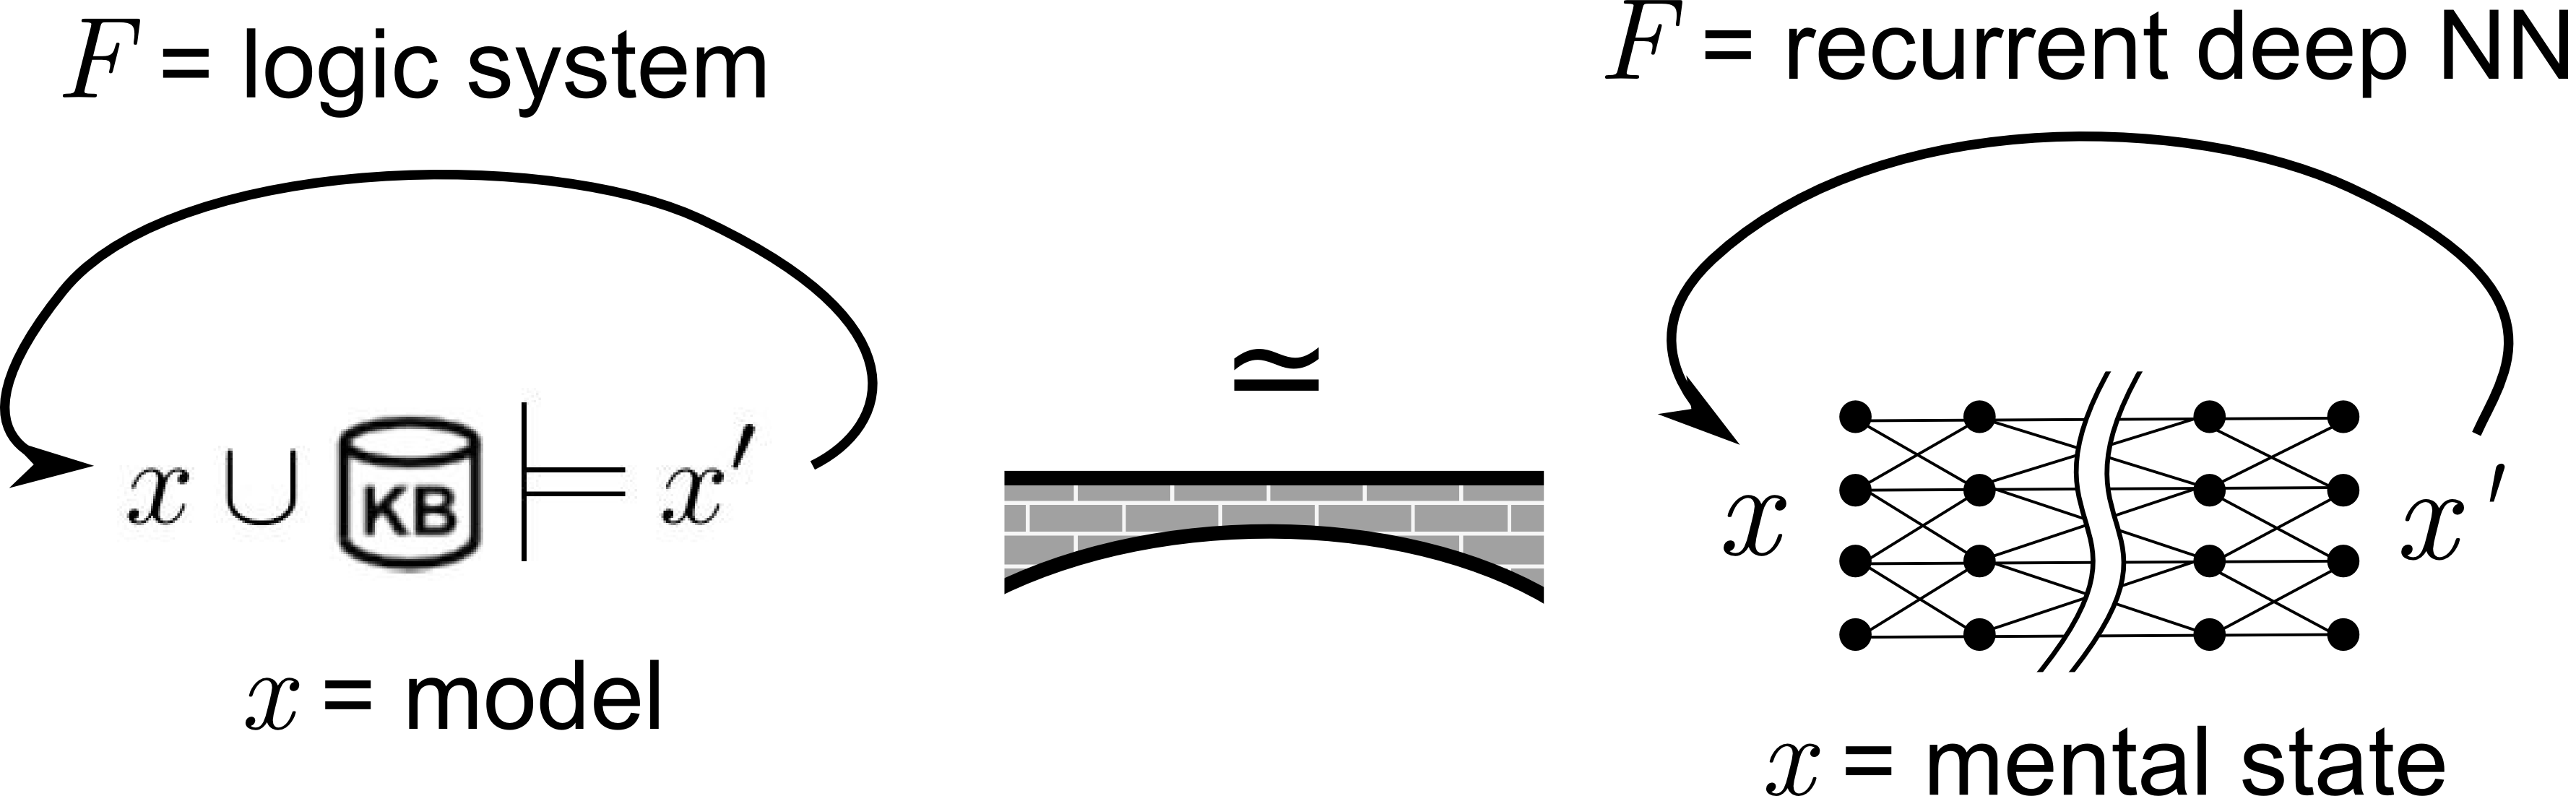
\includegraphics[scale=0.6]{bridge.png}
\end{equation}

I will first explain the structure of the neural side, then the structure of the logic side.
%首先解释 logic 那边的结构,然后再解释 neural network 那边的结构。

\section{The structure of neural networks}

A \textbf{neural network} is basically:
%一个\textbf{神经网络}基本上是:
\begin{eqnarray}
& \mbox{\footnotesize \textbf{weight} matrix } \tikzmark{weightMatrix} \mbox{\footnotesize for each layer} \quad \quad \mbox{\footnotesize total \# of layers} \tikzmark{numLayers} \nonumber \\
\nonumber \\
& F(\vect{x}) = \sigmoid(W_1 \tikzmark{wa} \sigmoid(W_2 \tikzmark{wb} ... \sigmoid( W_L \tikzmark{wc} \tikzmark{L} \; \vect{x} )))
\begin{tikzpicture}[overlay,remember picture]
  \draw[-, shorten <=17pt, transform canvas={shift={(-10pt,10pt)}}] (weightMatrix.center) to (wa.center);
  \draw[-, shorten <=21pt, transform canvas={shift={(-10pt,10pt)}}] (weightMatrix.center) to (wb.center);
  \draw[-, shorten <=33pt, transform canvas={shift={(-10pt,10pt)}}] (weightMatrix.center) to (wc.center);
  \draw (numLayers.center) +(-40pt,-5pt) -- ([shift={(-2pt,6pt)}]L.center);
\end{tikzpicture}
\end{eqnarray}
where $\sigmoid$ is the sigmoid function applied component-wise to each neuron (whose role is to provide \textbf{non-linearity}).

$\sigmoid$ acts on each component of $\vect{x}$;  Its action is \textbf{not invariant} under a change of coordinates.  Therefore, $\sigmoid$ is not a vector operation, and thus \uline{$\mathbb{X}$ is not a \textbf{vector space} structure}.  Common practice is to denote $\vec{x}$ as a vector, but this is misleading.
%$\sigmoid$ 作用在 $\vect{x}$ 的每个分量上,它的作用在座标变换下\textbf{没有不变性}。 所以 $\sigmoid$ 不是一个向量运算,从而 \underline{$\mathcal{X}$ 的结构也不是\textbf{向量空间}的结构}。 通常习惯把 $\vec{x}$ 写成向量形式,但这是误导的。

Consider, for example, to recognize \textit{``white cat chases black cat''}.  The \textit{``cat''} object has to be recognied twice;  Obviously we should not waste 2 neural networks to do this.  If we connect a neural network \textbf{head to tail}, we get a minimalist cognitive architecture with a \textbf{recurrent} loop:
\begin{equation}
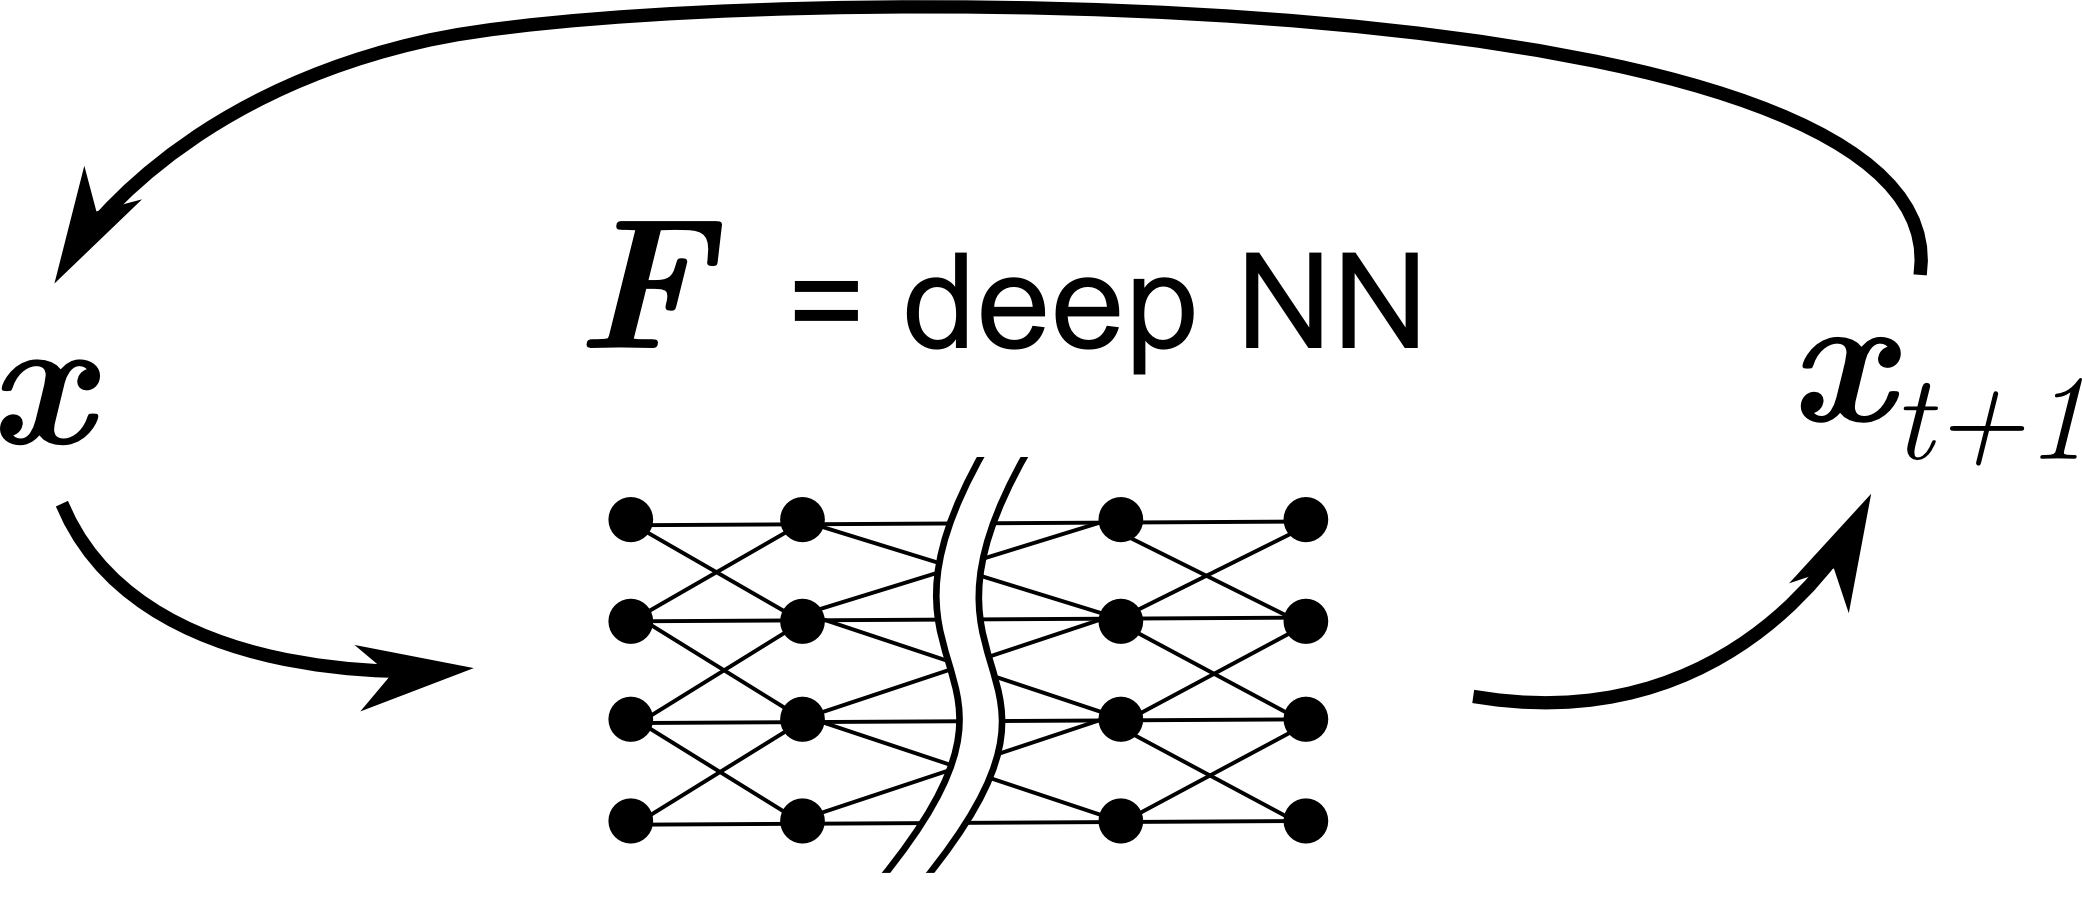
\includegraphics[scale=0.6]{genifer-model-00.png}
\end{equation}
Its state equation is:
\begin{eqnarray}
\boxed{\mbox{discrete time}} \quad \quad & \vect{x}_{t+1} = \vect{F}(\vect{x}_t) \label{eqn0}\\
\boxed{\mbox{continuous time}} \quad \quad & \dot{\vect{x}} = \vect{f}(\vect{x}) \label{eqn:continuous-time}
\end{eqnarray}
From this we can see that $\mathbb{X}$ is a \textbf{differentiable manifold}.  The deeper theory is that it is a Hamiltonian system, having a \textbf{symplectic} structure (cf. our first paper \cite{YanLabyrinth}).

\subsection{What are ``features''?}

Now let's think about how a neural network performs pattern recognition, perhaps it would be illuminating....
%现在思考一下,神经网络怎样识别模式,或许会有帮助:

Consider the simplest case, eg. a layer of neural network extracting visual features from the digit ``9''.  This layer may have many neurons (left figure), each neuron locally covers a region of the input layer, the so-called ``local receptive field'' in the neuroscience of vision (right figure).
%考虑最简单的情况,例如提取 digit ``9'' 的特徵的一层网络。 这层网络可以有很多神经元(左图),每个神经元局部地覆盖输入层,即所谓视觉神经元的 local receptive field(右图)。
\begin{equation}
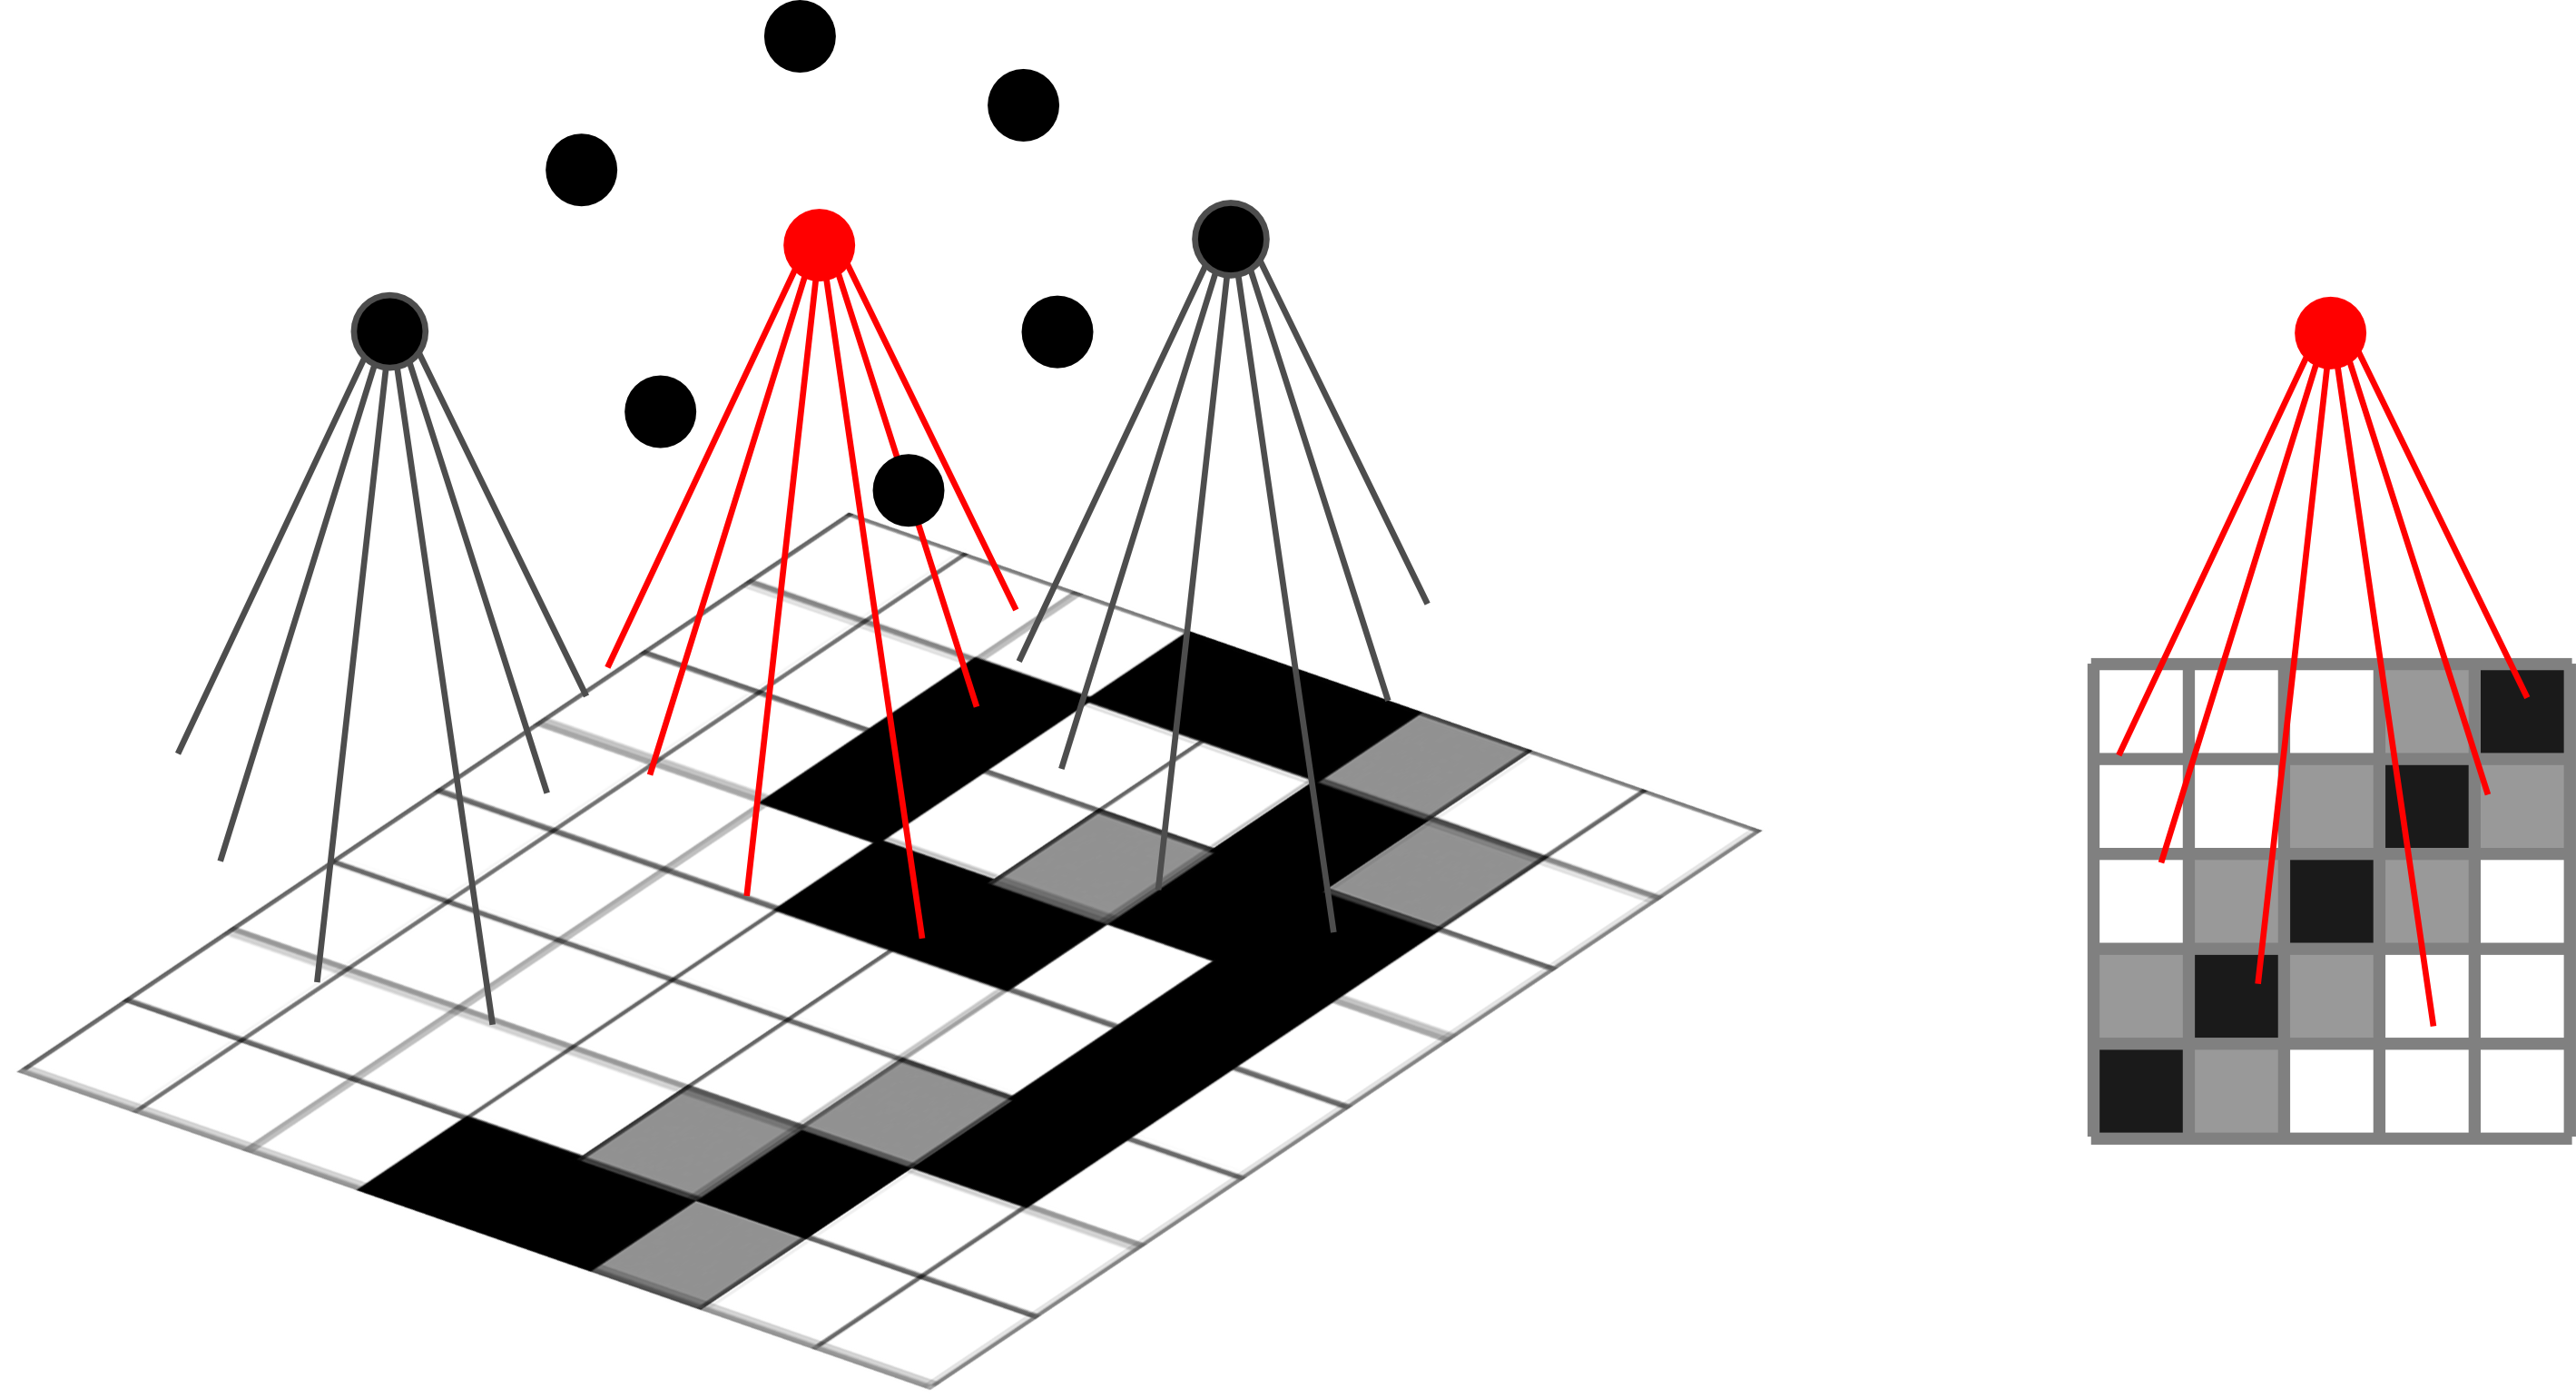
\includegraphics[scale=0.5]{feature-recognition.png}
\end{equation}
Suppose the red neuron is responsible for recognizing the ``diagonal line'' feature.  Its equation is $\vect{y} = \sigmoid (W \vect{x})$.  The matrix $W$'s role is to affine ``rotate'' the feature space, so that the features we desire is pointing in a certain direction.  Then we use $\sigmoid$ to ``\textbf{squeeze}'' the desired and undesired features.  The output after $\sigmoid$ represents the \textbf{presence or absence} of a particular feature, ie $\{0, 1\}$.  This is a form of information \textbf{compression}.

%更准确地说,特徵被挤压到 $[0,1]$ 区间内,资讯没有消失,但如果计算的\textbf{解析度} (resolution) 有限,资讯确实会损失的。 如果输出层有 $n$ 个神经元,它们能够代表的 distributive features 个数是 $[0,1]^n$。 这是连续统的 $n$ 次幂,但解析度令它变成是有限的。
From the above reasoning, we may draw a general principle, which I call the \textbf{Neural Postulate}:
\begin{equation}
\begin{array}{l}
\mbox{\textbullet \underline{Each neuron represents the presence or absence of a certain \textbf{feature}}}\\
\mbox{\textbullet \underline{Higher-layer neurons represents \textbf{relations} between lower-layer features}}
\end{array}
\end{equation}  

Following this line of thinking, we may conjecture this correspondence:
\begin{eqnarray}
\label{conclusion1}
\mathcal{M} & \quad \simeq \quad & \mathcal{X} \nonumber \\
\mbox{constant} \quad 
\includegraphics[scale=0.5]{node.png} & \quad \Leftrightarrow \quad & \mbox{neuron} \\
\mbox{relation} \quad 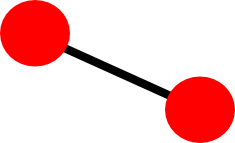
\includegraphics[scale=0.5]{link.png} & \quad \Leftrightarrow \quad & \mbox{relation between higher and lower neurons} \nonumber
\end{eqnarray}

%But beware that this correspondence may not be 1-1, it could be one constant corresponding to several neurons' (linear?) \textbf{combination}.  The actual situation may be illustrated as follows (each layer may contain a vast number of neurons):
%\begin{equation}
%\label{conclusion2}
%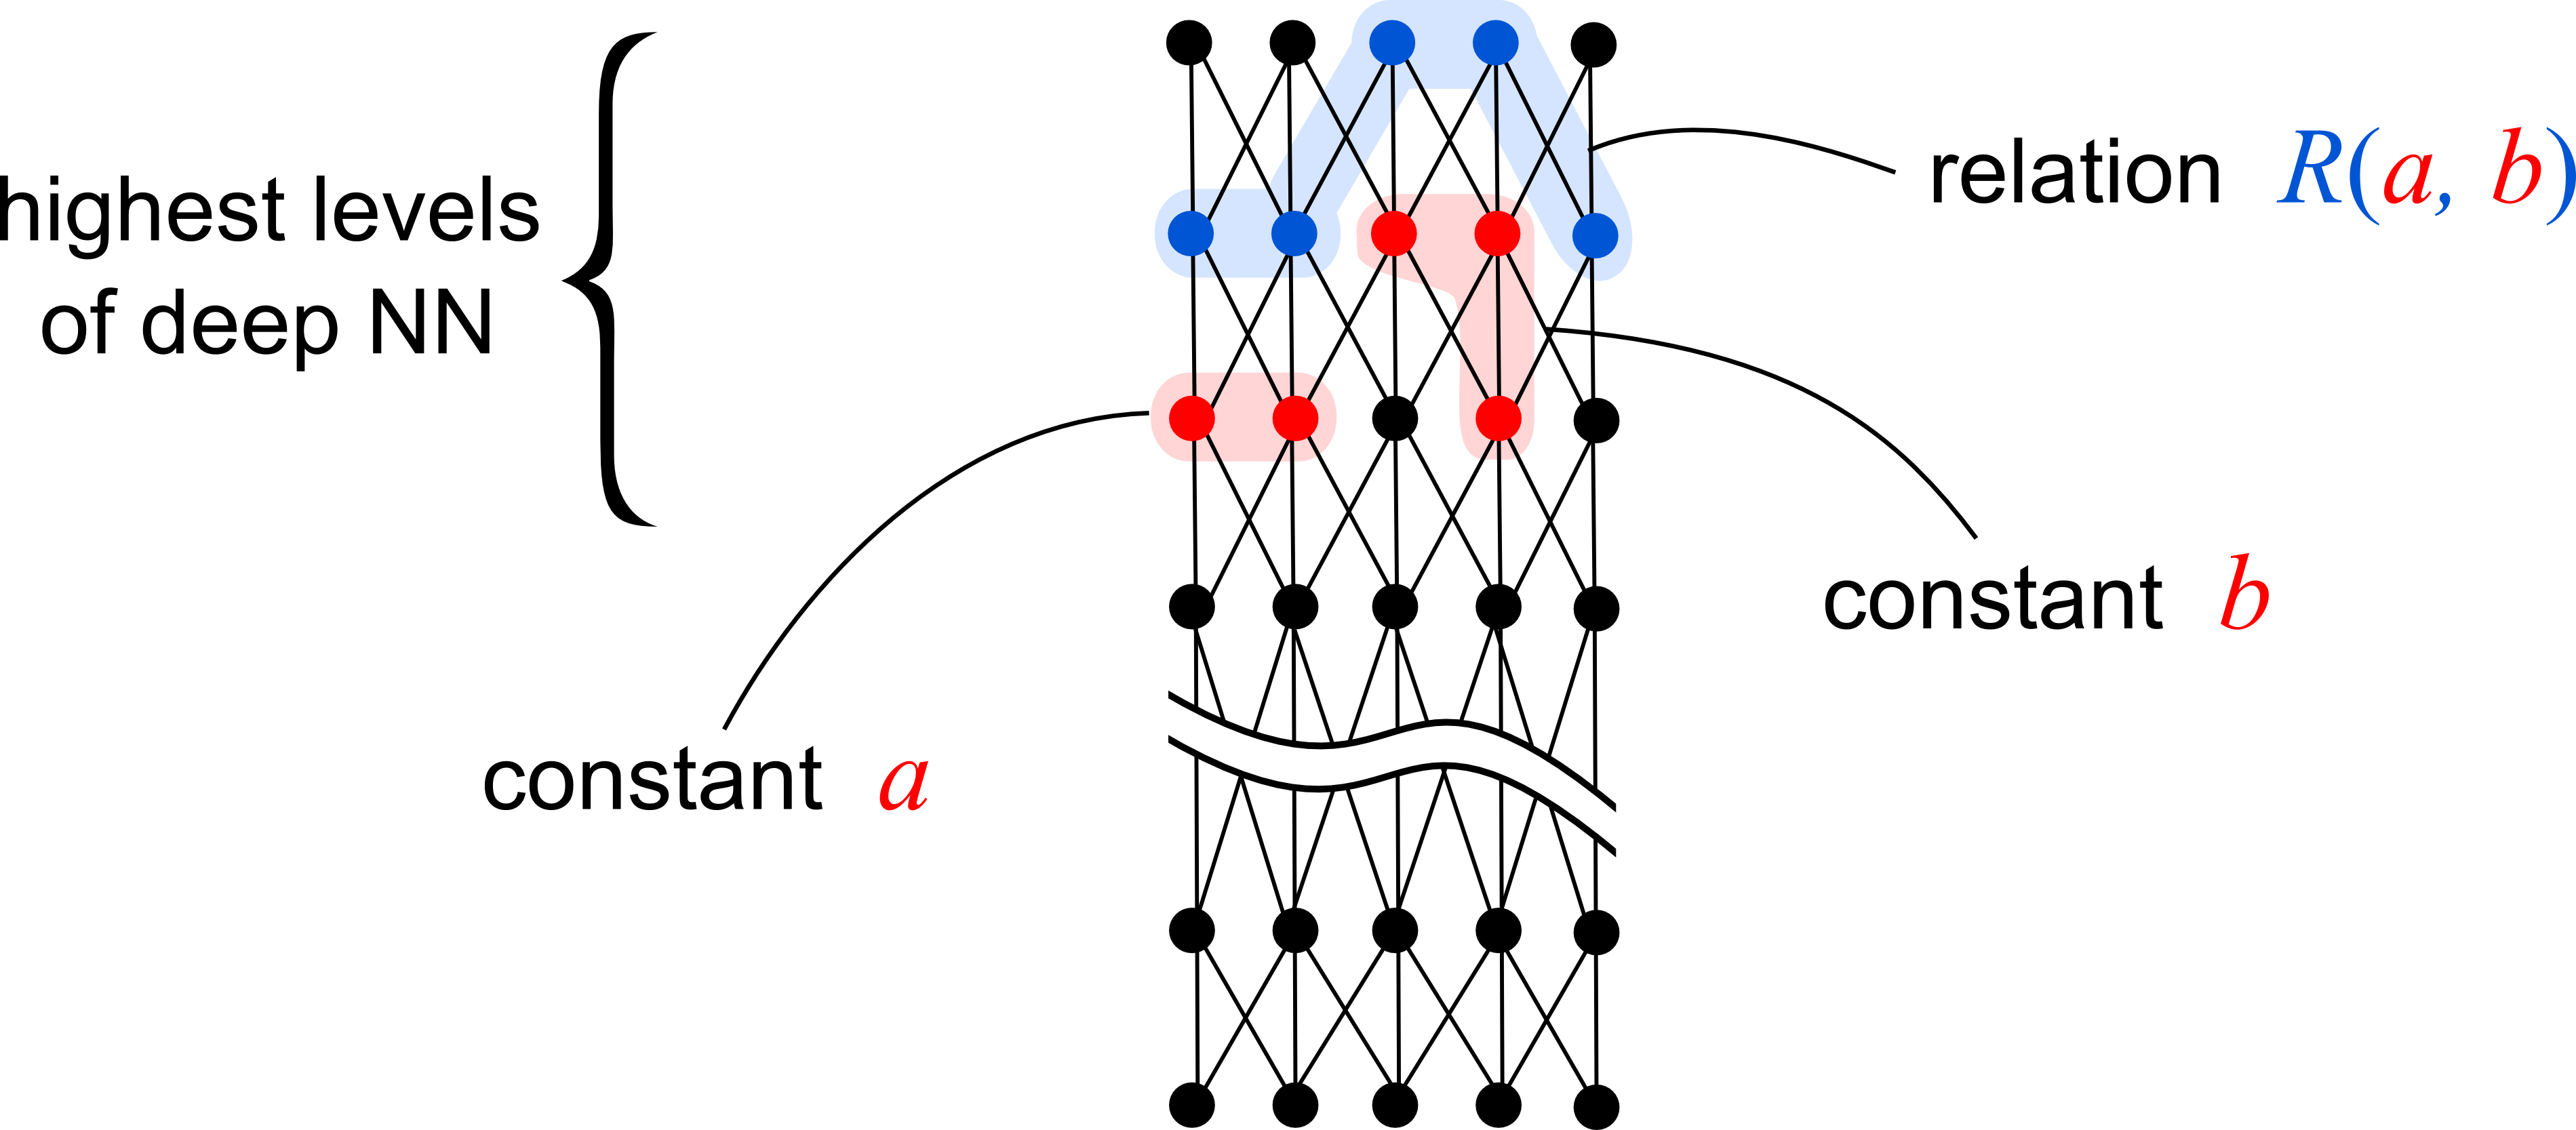
\includegraphics[scale=0.5]{actual-bridge.png}
%\end{equation}
%$R(a,b)$ can be searched for among the \textbf{common parents} of $a, b$ (eg. those blue neurons;  The value of $R(a, b)$ = a certain linear combination of blue neurons).  This can be verified by the condition:  If the signals of $a$ and $b$ are both ``present'', the value of $R(a, b)$ should also be ``true''.

The following cartoon illustrates this correspondence from the perspective of \textbf{model theory}:
\begin{equation}
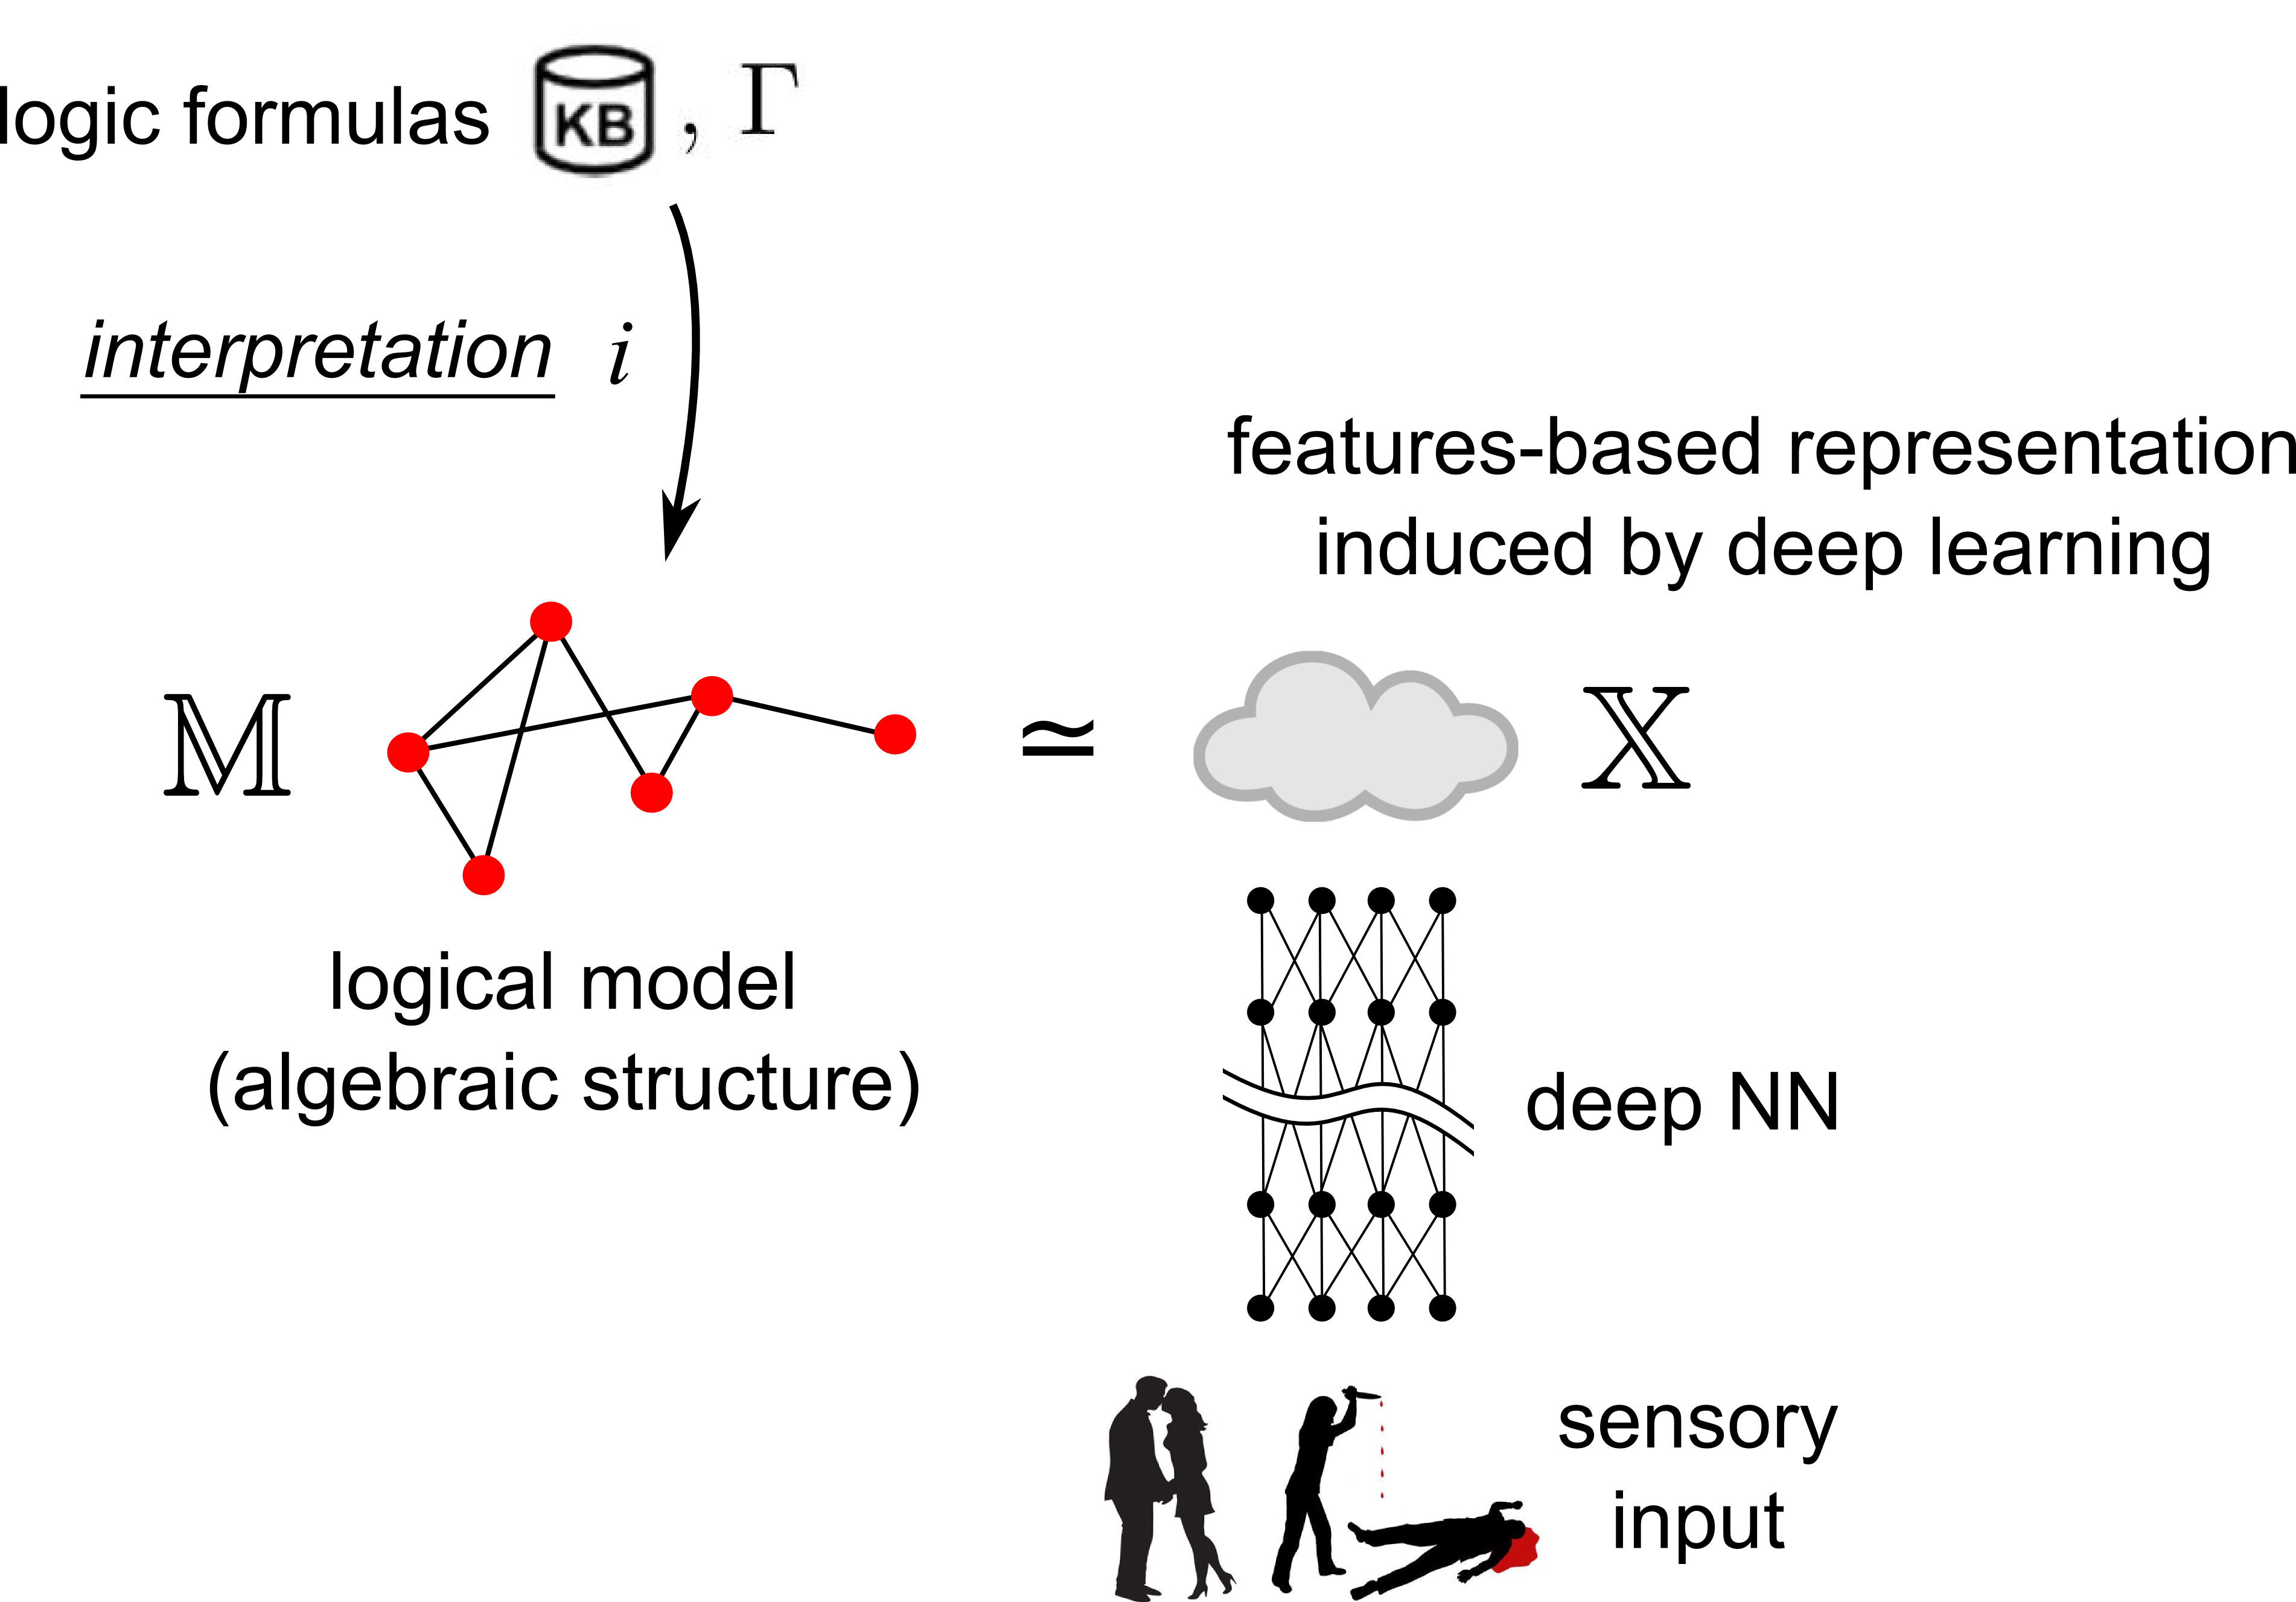
\includegraphics[scale=0.75]{model-theory-cartoon.png}
\end{equation}

\begin{tcolorbox}[breakable, enhanced]

\textbf{A little digression on chaos theory:}

The role of $\sigmoid^{-1}$ is to ``stretch'', dragging points that are close neighbors to more distant positions.  Looking at the common \textbf{threshold functions}, we see they are all non-linear \textbf{deformations} away from the identity $y = x$:
\begin{equation}
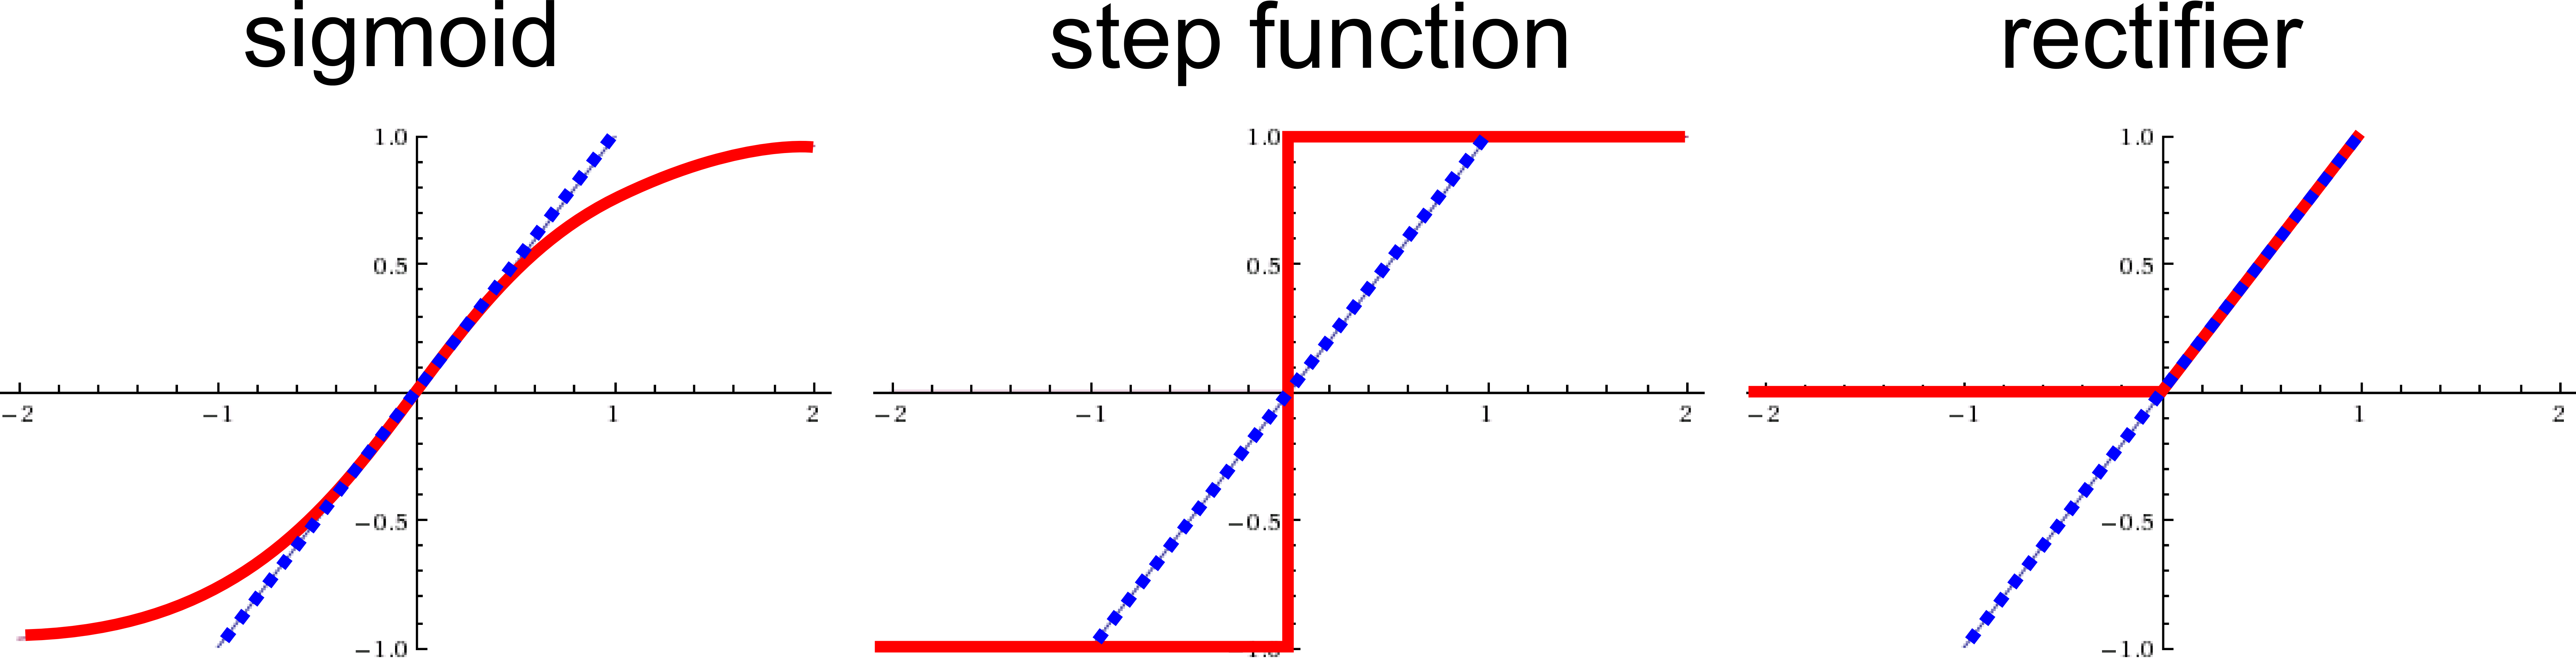
\includegraphics[scale=0.25]{activation-functions.png}
\end{equation}
This is very similar to the ``horseshoe'' proposed by Steven Smale \cite{Smale1967}, a recipe for creating chaos.  A variant of the Smale horseshoe is the ``baker map'', analogous to kneading dough in bakery.  ``Stretching'' and then putting back to the original space, and repeating this process, creates chaos \cite{Gilmore2011} \cite{Tel2006}.  

%There is something of significance here: $\vect{F}^{-1}$ has the typical characteristic of chaos: the ``sensitivity to small changes in initial conditions''.  According to my view, the forward propagation of a neural network performs pattern recogntion = \textbf{information compression}, and backward is de-compression.  While operating backwards, a single output value may correspond to many different inputs ($\vect{F}^{-1}(\vect{x})$ can be many patterns), thus small changes in the ouput (eg 0.99 and 0.98) will cause $\vect{F}^{-1}$ to fluctuate wildly, ie, chaos.  That means the inverse $\vect{F}$ is \textbf{unpredictable}, or to put it succinctly:  the forward neural network $\vect{F}$ is an \textbf{irreversible} compression process.

%The recent example of DeepDream \cite{wikiDeepDreaming} that generates ``psychedelic'' images using the $\vect{F}^{-1}$ pre-image serves as evidence that $\vect{F}^{-1}$ could be wildly different from the original image:
%\begin{equation}
%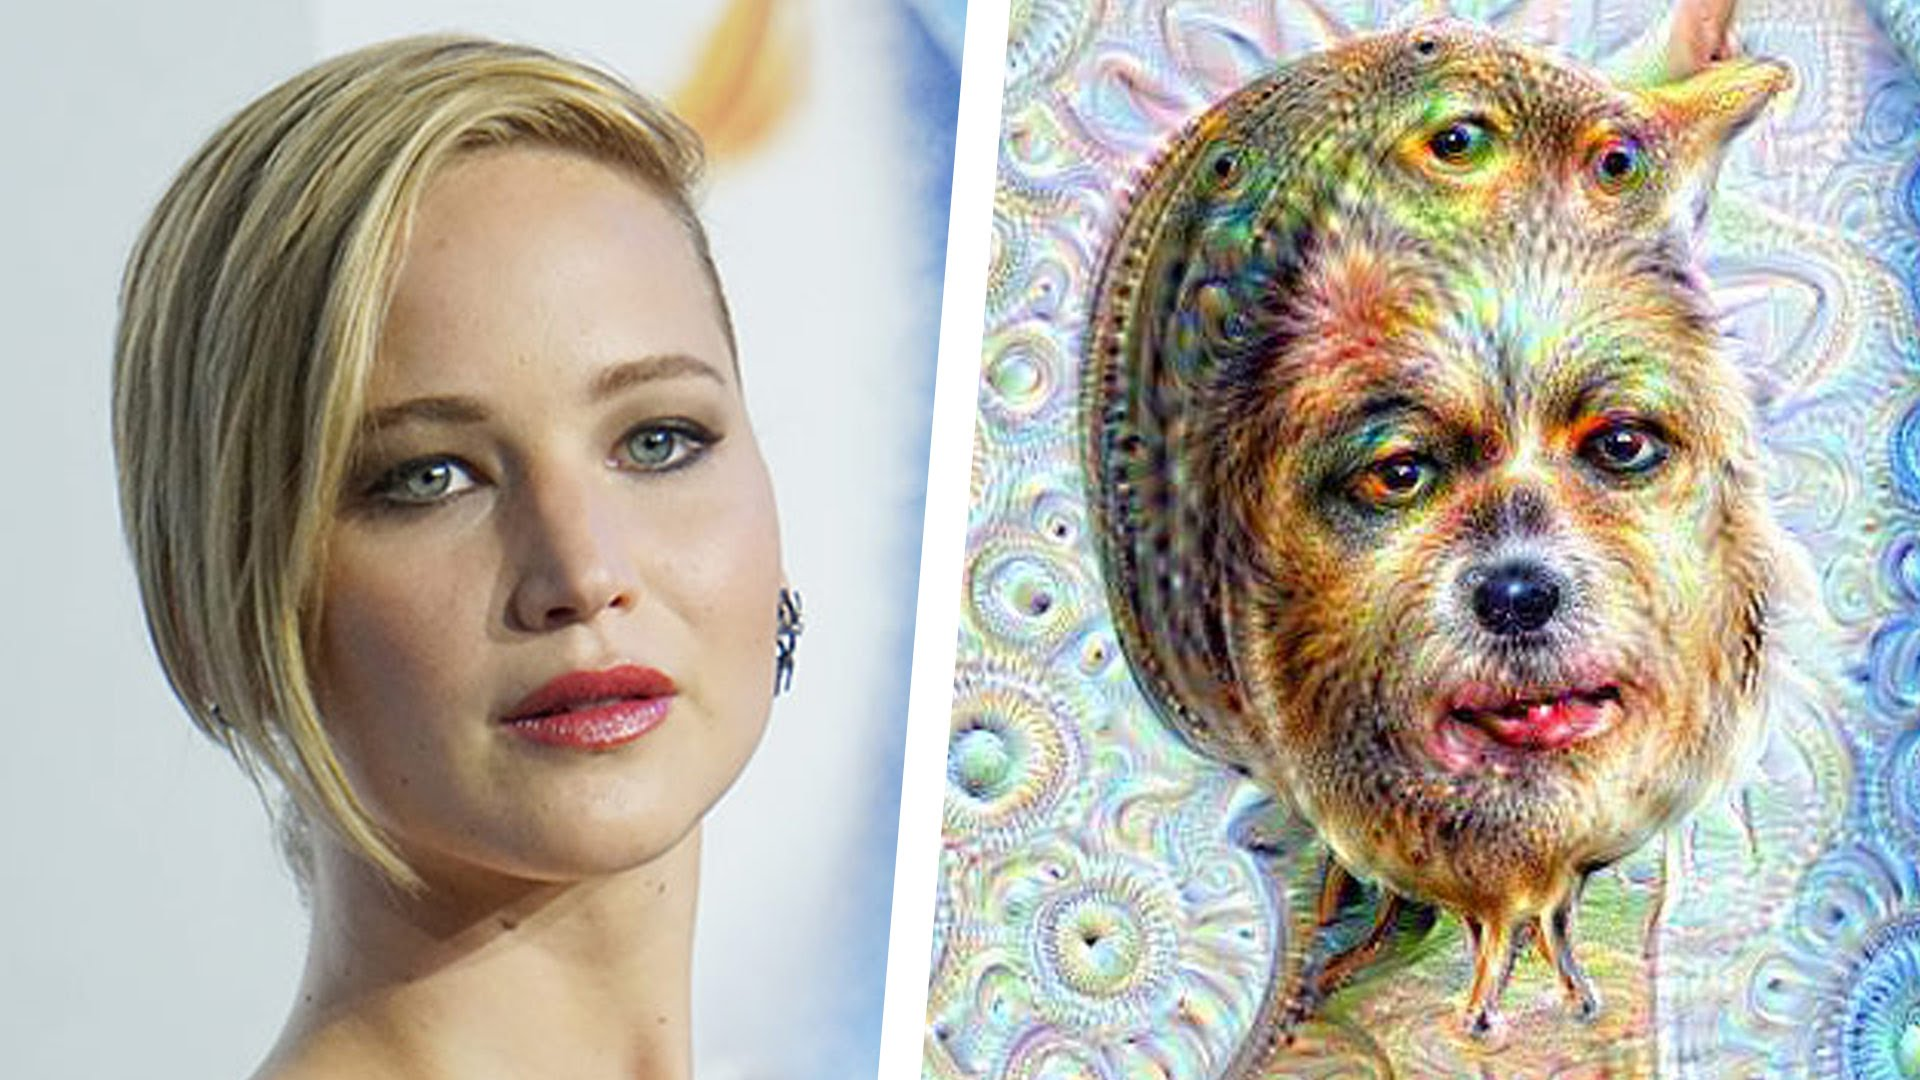
\includegraphics[scale=0.09]{neuromorphic-art.jpg}
%\end{equation}

%In forward mode there does not exist this kind of ``stretching'', which seems to imply that chaos would be absent.  Also, according to the contraction mapping theorem, the iteration of $\vect{F}$ will terminate at fixed point(s), provided that $\vect{F}$ is contractive, ie, the spectral radius of the Jacobian matrix of $\vect{F}$ $\le 1$, but this latter point is not yet confirmed (indeed, if $W$ is unconstrained, it seems not to hold).

%Time-reversal of chaos is not necessarily chaotic.  However, in ergodic theory one can calculate the \textbf{topological entropy} which is time-reversal invariant.  I am not sure if other measures of entropy might explain the irreversibility (may need to consult some experts in ergodic theory....)

\end{tcolorbox}

\section{Structure of logic}

A \textbf{logic system} can be defined as:
\let\labelitemi\labelitemii
\begin{itemize}
\item a set of symbols for \textbf{constants}, \textbf{predicates}, and \textbf{functions}
\item \textbf{propositions} built from the above atoms
\item \textbf{connectives} between simple propositions, eg:  $\neg, \wedge, \vee$
\item The \textbf{logical consequence} relation: $\Gamma \vdash \Delta$
% \item 命题的内部结构(命题由概念原子组合而成)
\end{itemize}

The learning algorithm for logic-based AI is studied under the topic of ILP (inductive logic programming), which is a well-established field (cf. my tutorial \cite{YanILPtutorial} or de Raedt's textbook \cite{DeRaedt2008}).  ILP performs \textbf{combinatorial search} in the symbolic space of logic formulas, and is very slow.  The gradient descent of neural networks is much faster.  In the following we examine the prospects of combining these 2 approaches.

%From raw sensory data, we can \textbf{inductively} learn a set of logic formulas, ie. the knowledge base $\KB$.  This process is under the research heading of \textbf{inductive logic programming} (ILP).  Everyone familiar with classical AI knows ILP, but in recent decades the popular focus is on \textbf{statistical learning}, and this kind of symbolic logic learning is relatively neglected.
%由一些原始的 sensory data,可以透过逻辑学习出一些 logic formulas,即知识库 (knowledge base) $\KB$。 这个过程叫逻辑\textbf{诱导学习} (inductive logic programming, ILP)。 学经典 AI 的人都知道 ILP,但近数十年来,注意力集中在统计学习,这种符号逻辑的学习法被忽视。 

%Raw sensory data can be processed using neural-based pattern recognition, or it can be processed via ILP-based pattern recognition.  The result of these two pathways should obviously be isomorphic (at least approximately):
%\begin{equation}
%\begin{tikzcd}[]
%\mbox{Logic representation} \arrow[rr, phantom, "\simeq"] & & \mbox{Neural representation} \\
% & \arrow[ul, "\mbox{inductive logic learning}"] \arrow[ur, "\mbox{deep NN learning}" swap] %
\includegraphics[scale=0.5]{sensory-data.png} &
%\end{tikzcd}
%\end{equation}

%I have spent a lot of time thinking how to transition logic-based representations to the neural side, but found this target to be very elusive.
%我以前花了很多时间思考怎样将逻辑的 representation 过渡到神经网络去,但发觉这个目标非常 elusive。

%On the one hand, logic is the study of the laws of human thinking, developed over centuries.  The logical description is correct;  There should be a correspondence between logic and neural, as they are both doing the same thing (intelligence).
%一方面,逻辑是几百年来发展起来的关於人类思考的规律; 逻辑的描述是正确的; 逻辑和神经之间必然有一个 correspondence,因为它们都在做同样的事(智能)。 

%In \textbf{cognitive science}, many researchers believe the representations inside our brains are so-called ``mental models'', and few would believe that the brain uses a representation like the propositions in symbolic logic, or to think with the sort of symbolic manipulations as $\lambda$-calculus.
%在\textbf{认知科学}里,有很多人相信大脑的内部的 representation 是一些所谓 ``mental models'',而很少人会相信大脑使用一些像命题那样的符号结构做 representation,甚至用 $\lambda$-calculus 那样的符号 manipulation 去思考。

%As an example, when we verbally describe a case of murder, the reader would establish in her mind's eye a ``model'' that is similar to real experience yet is unreal.  The human brain seems to use such mental models to think, rather than with a bunch of propositions.  Examples of model-based reasoning using logic are \cite{Magnani1999} \cite{Magnani2002}.
%举例来说,用文字描述一起凶杀案,读者心目中会建立一个「模型」,它类似於真实经验但又不是真实的。 人脑似乎是用这样的 mental models 思考,而不是一些命题的集合。 %至於 mental models 是什么,目前认知科学还未有定论。

%So eventually I realized that the logic-neural correspondence must be achieved through model theory:
%\begin{equation}
%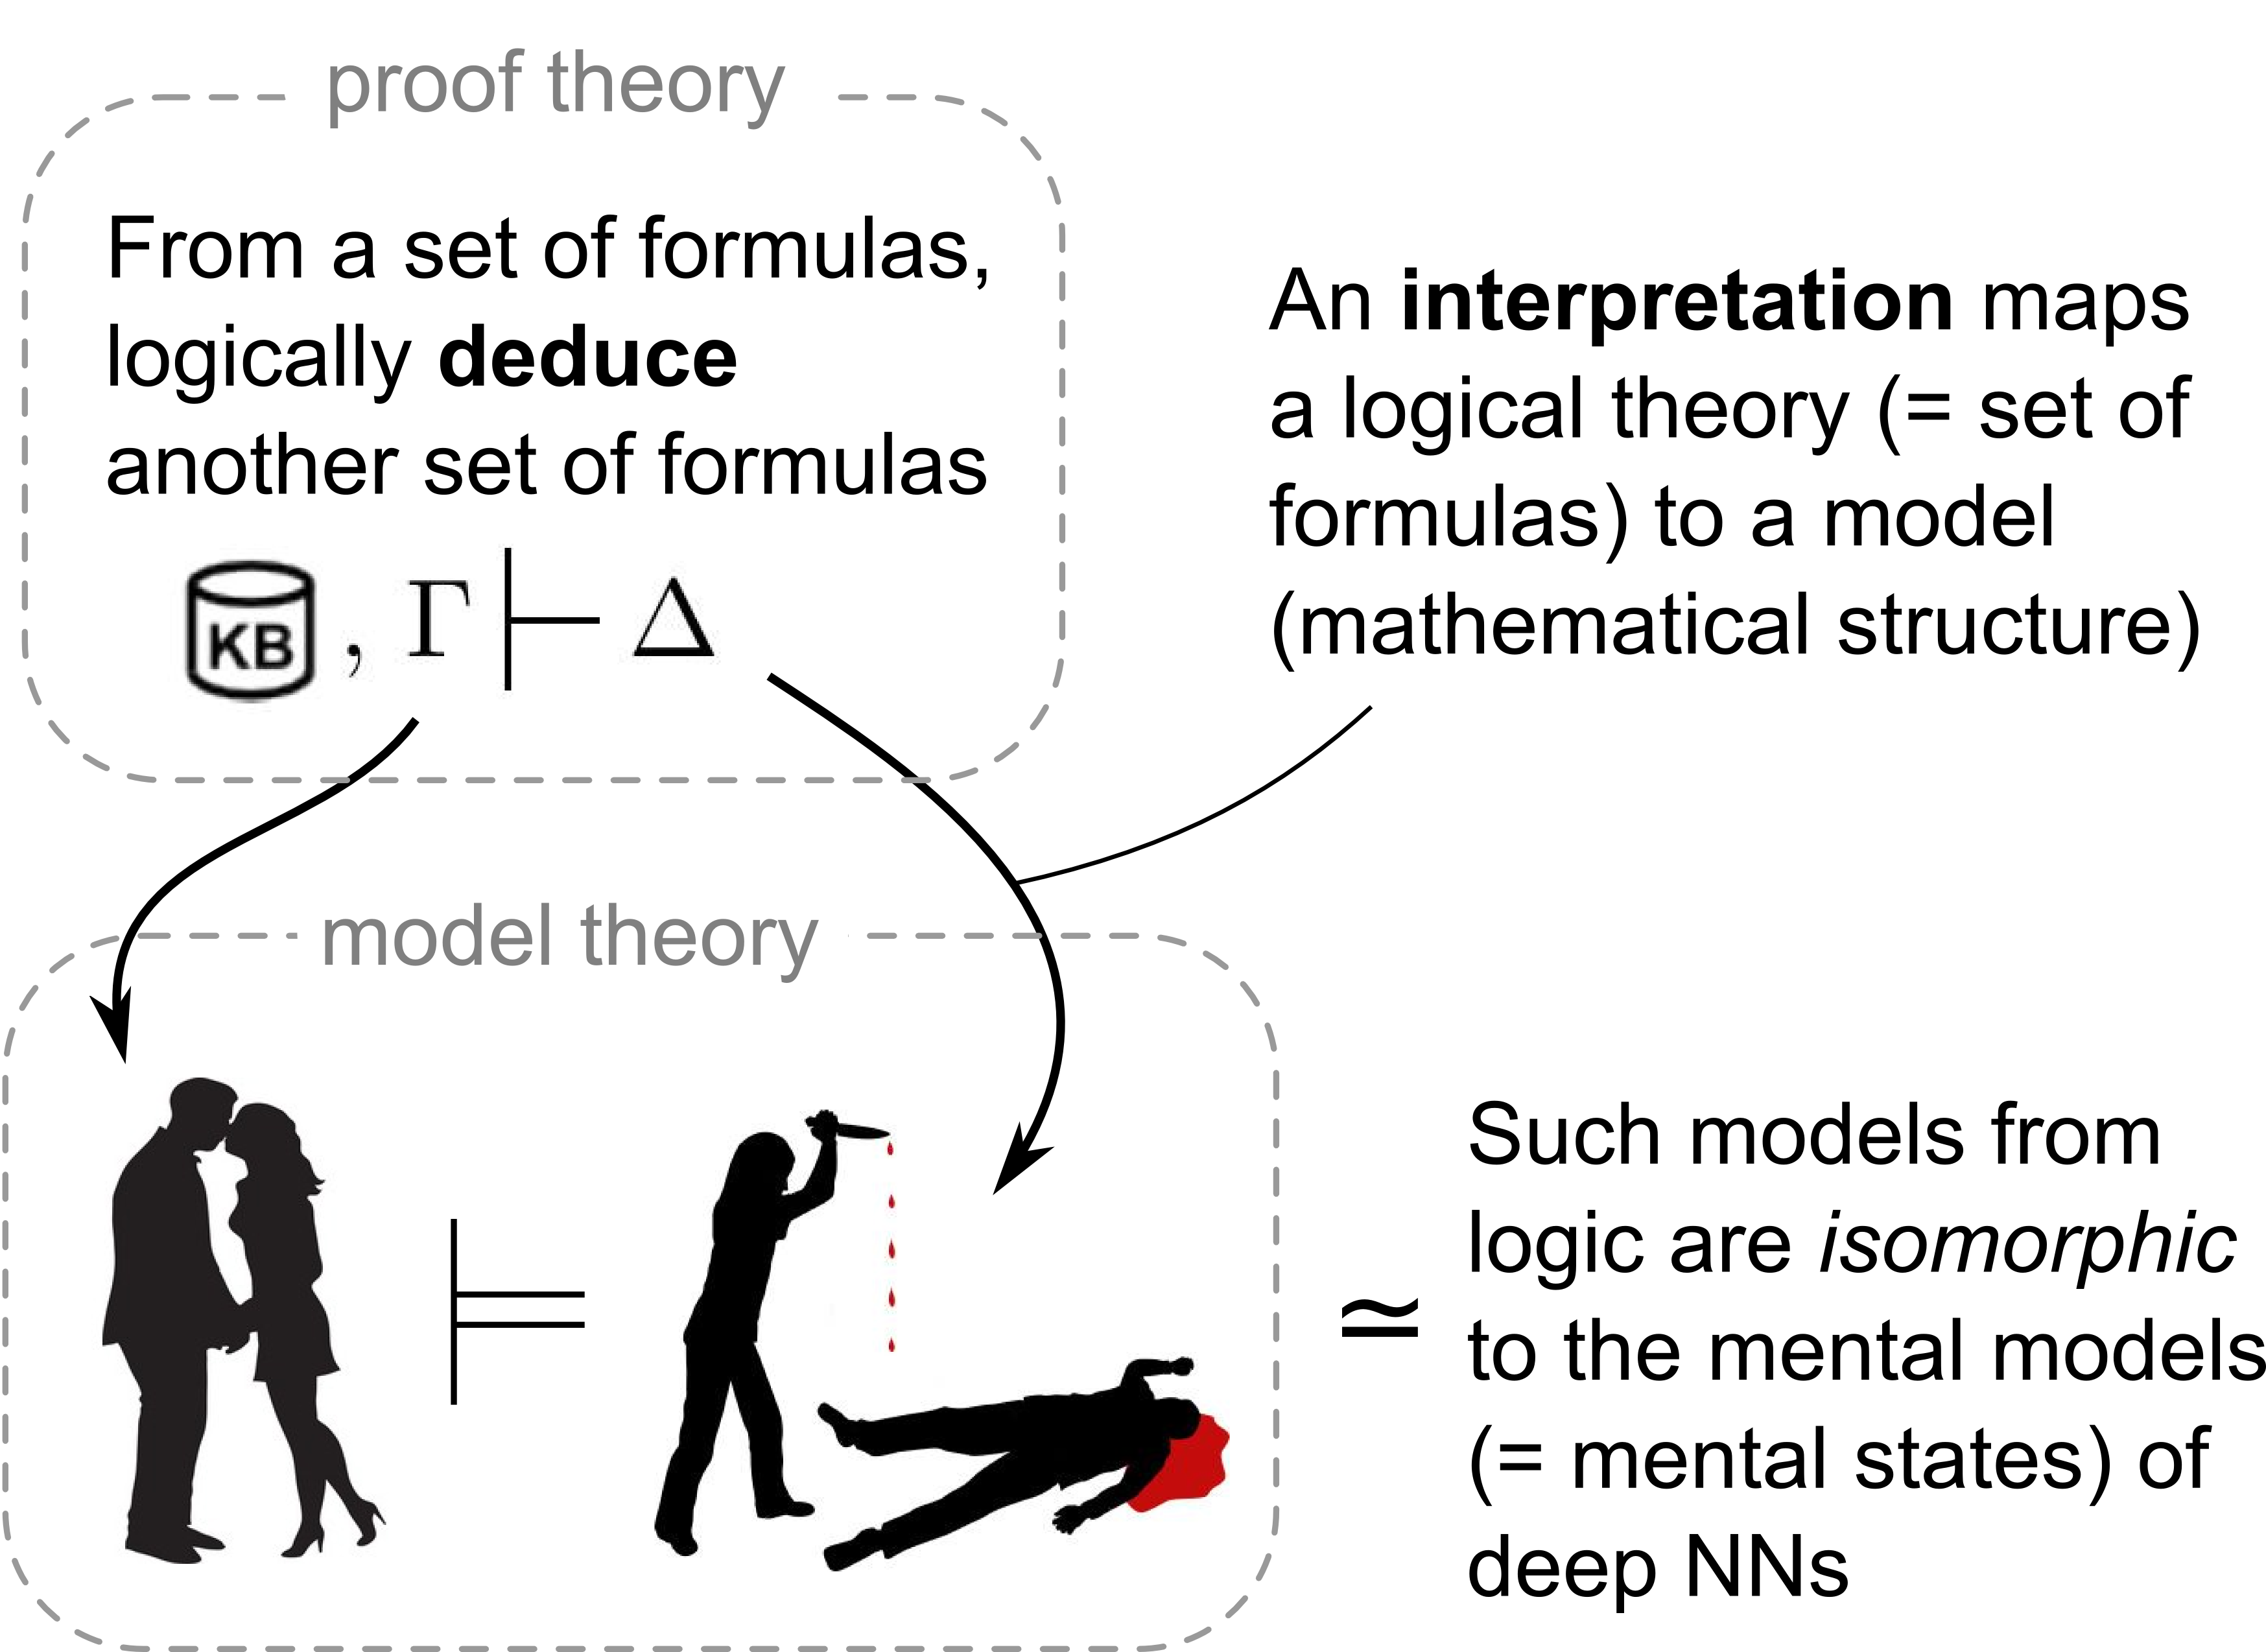
\includegraphics[scale=0.75]{model-theory.png}
%\end{equation}

%$\vdash$ means deducing from a set of (symbolic logic) \textbf{formulas} to new formulas.  $\vDash$ means that a \textbf{model} necessarily entails another model.

% \footnote{Knowledge-based model construction (\textbf{KBMC}) 这个术语较少人知道,但其实是最关键的结构; 换句话说,就是从 $\KB$ 中抽出一组命题 $\Gamma$,去\textbf{组合}一个 model 或 proof tree,而这个 proof tree 的某个节点,就是新的结论。 亦即 $\Gamma \vdash Q$。 KBMC 的概念适用於经典逻辑也适用於 Bayesian networks。}

Our idea is to transfer the structure of logic to neural networks.  The logic structure can be broken down into:
\begin{itemize}
\item propositional-level structure \\
(the mental state $\vect{x}$ is represented as a \textbf{set} of propositions $p_i \in \vect{x}$)
\item sub-propositional structure
\end{itemize}

\subsection{Propositional-level structure}

\subsubsection{Decomposition of the mental state into propositions}

The mental state $\vect{x}$ may be broken down into a conjunction of propositions:
\begin{equation}
\vect{x}_1 = \mbox{ I'm attending a seminar } \wedge \mbox{ I feel hungry } \wedge ....
\end{equation}
There could be another mental state:
\begin{equation}
\vect{x}_2 = \mbox{ I'm riding the subway } \wedge \mbox{ I feel hungry } \wedge ....
\end{equation}
It would be very inefficient if $x_1$ and $x_2$ are considered completely different states (without decomposition).

\subsubsection{Boolean algebra}

A \textbf{Boolean algebra} is a structure with:
\begin{eqnarray}
& \mbox{\footnotesize underlying set} \tikzmark{underSet} \quad \mbox{\footnotesize binary ops} \tikzmark{binaryOps} \quad \mbox{\footnotesize unary op} \tikzmark{unaryOp} \nonumber\\
\nonumber \\
& \mathcal{B} = ( \, \tikzmark{UnderSet} A, \tikzmark{BinaryOps} \overbrace{\wedge, \vee}, \tikzmark{UnaryOp} \neg \, )
\begin{tikzpicture}[overlay,remember picture]
  \draw (underSet.center) +(-35pt,-4pt) -- ([shift={(3pt,11pt)}]UnderSet.center);
  \draw (binaryOps.center) +(-29pt,-3pt) -- ([shift={(13pt,14pt)}]BinaryOps.center);
  \draw (unaryOp.center) +(-30pt,-3pt) -- ([shift={(4pt,11pt)}]UnaryOp.center);
\end{tikzpicture}
\end{eqnarray}
From my experience in logic-based AI, the most essential aspect of the Boolean structure (especially after introducing fuzzy-probabilistic reasoning) is this \textbf{commutativity} relation:
\begin{equation}
\forall a,b \in \mathcal{B}.  \quad \quad a \wedge b = b \wedge a
\end{equation}

\subsubsection{Mapping propositions $\rightarrow$ vector space}

\textbf{Our gaol:} map a set of propositions (\textit{order is unimportant}) to a vector space.

Consider the simplest situation:  $P_1$ and $P_2$ are two \textbf{containers} for propositions, the mental state is $(P_1, P_2)$.  Each proposition can be either $A$ or $B$.  We can arrange the placement of elements of $P_1 \times P_2$ in this way:
\begin{equation}
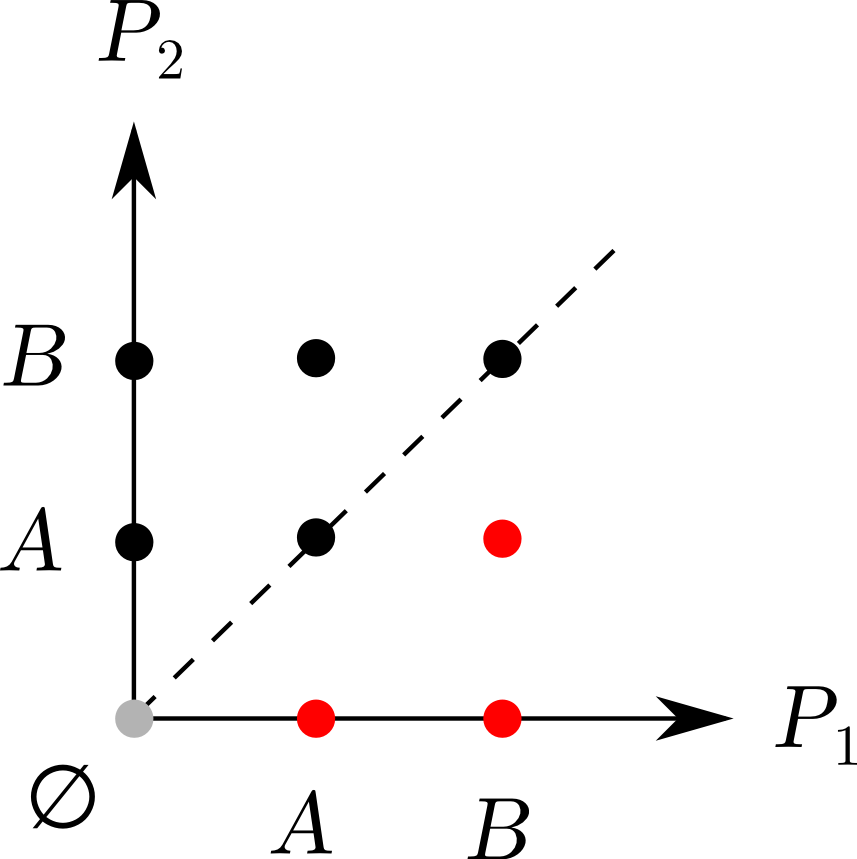
\includegraphics[scale=0.75]{lower-triangular.png}
\end{equation}
For example, the 3 {\color{red}red} dots in the lower triangle $\halfsquare$ represent $\{ A \}$, $\{ B \}$, and $\{ A, B \}$.  The diagonal elements are not needed, because $(A, A)$ etc. are \textit{redundant} repetitions.  In other words, all the propositional combinations are:
\begin{equation}
\halfsquare \; \setminus \mbox{ diagonal } \cup \; \emptyset
\end{equation}
More abstractly, elements in this ``symmetric space'', eg. $(p_1, p_2, ..., p_n)$, are \textit{invariant} under actions of the \textbf{symmetric group} $S_n$, $n$ is finite.

In high dimensions, this space-saving scheme is extremely efficient:  After symmetrization, a ``corner'' of the hypercube has a volume that is only $1/n!$ of the original cube, eg. $n = 3$:
\begin{equation}
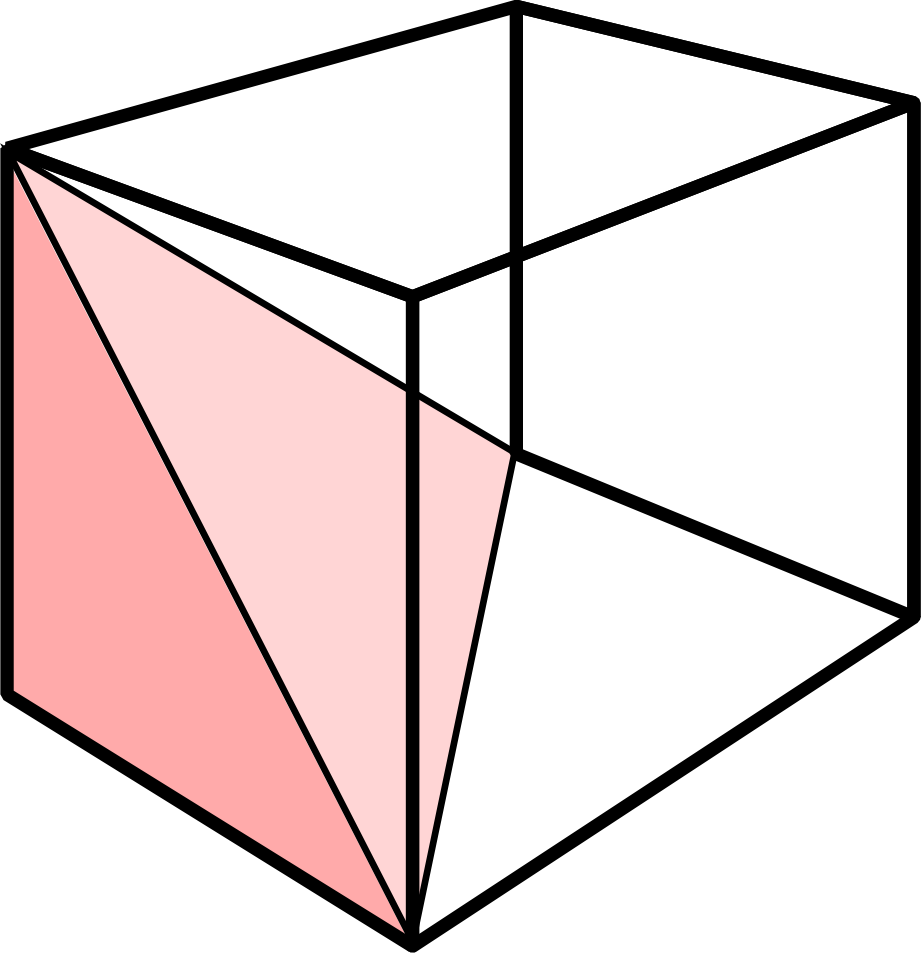
\includegraphics[scale=0.5]{cube-corner.png}
\end{equation}
Even as the \textbf{curse of dimensionality} grows exponentially, $n!$ is well sufficient to offset it.

Now consider the \textbf{functions} that live on this symmetric space;  How are their structures affected?  Before symmetrization, the functions have domains:
\begin{equation}
\vect{F}: \mathbb{X} \rightarrow \mathbb{X} \quad = \quad \mathbb{P}^n \rightarrow \mathbb{P}^n
\end{equation}
where $\mathbb{P}$ is the space of a single proposition.  After symmetrization:
\begin{equation}
\vect{F}: \mbox{sym}(\mathbb{P}^n) \rightarrow \mbox{sym}(\mathbb{P}^n) \quad = \quad \halfsquare \rightarrow \halfsquare
\end{equation}
The symmetric space $\mbox{sym}(\mathbb{P}_1, \mathbb{P}_2, .... \mathbb{P}_n)$ possesses an \textbf{order}.  That is to say, if the input to a function is $(p_1, p_2, ... , p_n)$, we need to \textbf{sort} the $p_i$'s according to a certain order on $\mathbb{P}$, before calling $\vect{F}$ to calculate.

Sorting in $\mathbb{P}$ is simple, because each $p \in \mathbb{P}$ already has a \textbf{location} in vector space (that is learned via deep learning).  $p_1 > p_2$ can be defined by a \textbf{cone} in the vector space, and then the order in $\mathbb{P}^n$ can be given by \textbf{lexicographic ordering}.

When implementing with as a neural network $\NN: \mathbb{R}^n \rightarrow \mathbb{R}^n$, we can keep the entire network, using only $\halfsquare$ as its domain and co-domain.  It seems that we have gained nothing, but consider if we train the network with 100 samples on $\halfsquare$ versus the whole hypercube.  $\halfsquare$ will receive the ``full strength'' of the data set whereas the hypercube will have its ``firepower'' diluted by $n!$.

%The algorithm in this section is very simple, yet it can achieve a $1/n!$ improvement.  It is very worth implementing to see its actual performance $\smiley$

\subsection{Sub-propositional structure}

This part is more complicated.  Traditionally the structure of predicate logic is so esoteric from the point of view of mathematics that it hindered the progress of logic and logic-based AI.

\subsubsection{Semantic distance and failure of compositionality}

Word2Vec\cite{Mikolov2013} embeds words into vector space with ``semantic distance'':
\begin{equation}
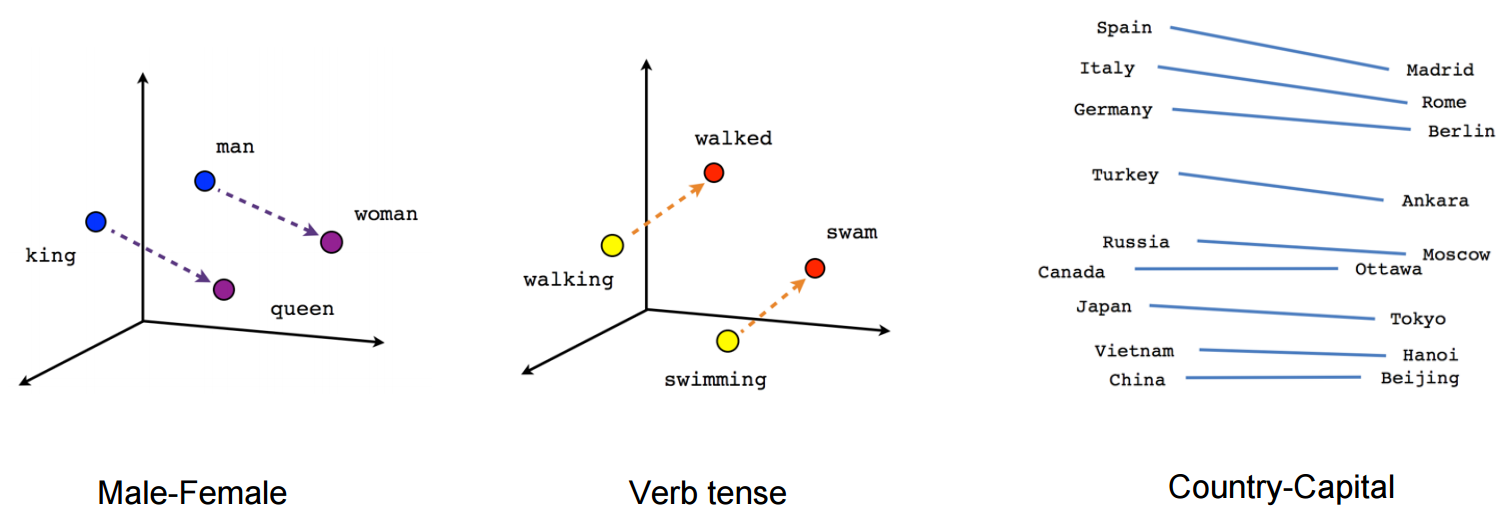
\includegraphics[scale=0.3]{word2vec-relations.png}
\end{equation}

After Word2Vec, a natural next step is to represent \textbf{sentences} with semantic distance.    One popular approach (eg \cite{Coecke2010}) is via \textbf{tensor products}.  For example:
\begin{equation}
\mbox{\textit{``I love you''}} \quad \Rightarrow \quad \mbox{i} \otimes \mbox{love} \otimes \mbox{you}
\end{equation}
but this approach has serious problems:  For example, pronouns such as ``you'' refer to various entities and must be resolved using rather complicated procedures, known as ``abductive interpretation'' in logic-based AI.  Without such interpretations the word-entity correspondence becomes very inaccurate.

\subsubsection{A logic based on ``features''}

Assuming that the compositionality problem can be bypassed, perhaps with logical atoms referring directly to entities (no pronouns, metaphors, etc), we may represent sentences by a ``conjunction'' of features (different from the $\wedge$ for propositions), eg:
\begin{eqnarray}
\vect{x} &=& \textit{I feel hungry} \nonumber \\
 &=& \textit{me} \cap \textit{physiology} \cap \textit{food} \cap \textit{negative-emotion} \cap .... 
\end{eqnarray}
This is like using a series of binary choices (= features) to determine an idea, like the game ``20 Questions''.

\subsubsection{OpenCog's logic based on hypergraphs}

To represent a complex scenario with many inter-relations, without using pronouns, perhaps \textbf{hypergraph} is a good choice.  This is the idea behind \href{http://wiki.opencog.org/w/The_Open_Cognition_Project}{OpenCog}'s representation.

A hypergraph is also called a ``set system''.  Any hypergraph can be represented as a set of edges, each edge being an element of the power set of the nodes.  Eg:
\begin{equation}
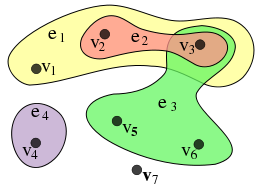
\includegraphics[scale=0.6]{hypergraph-wikipedia.png}
\end{equation}
This representation is convenient for our purpose:  Each edge can be represented as 1 proposition.  The mental state $\vect{x}$ = a hypergraph = a set of propositions.  We can use the symmetric space proposed above to represent the mental state.

Each proposition (edge) is a product of atomic concepts (nodes), we may further fix \#(nodes) per edge to, say, 3:
\begin{equation}
\boxed{\mbox{proposition}} \quad \vect{p} = c_1 \; c_2 \; c_3
\end{equation}
For example $c_1 \; c_2 \; c_3$ could be like subject-verb-object in natural language, where $c_1$ and $c_3$ are from the set of nouns / entities;  $c_2$ from the set of verbs / relations.  We don't need to be very precise about this, as the actual representation can be figured out via machine learning.  This is the age of \textit{post-modern}\footnote{With ``modern'' meaning ``structuralist'', as in designating structural elements such as ``NP (noun phrase)'' in phrase-structure grammar or the ``is-a'' link in old-fashioned AI.} AI!

\subsubsection{``Linkage'' phenomena in predicate logic}

Next we consider \textbf{variable substitution}, a key feature of predicate logics.  For example:

\begin{equation}
\forall X \; \forall Y \; \forall Z.  \quad  \text{grandfather}({\color{red}X} \tikzmark{x}, {\color{red}Z} \tikzmark{z}) \leftarrow \text{father}({\color{red}X} \tikzmark{p}, {\color{red}Y} \tikzmark{y}) \wedge \mbox{father}({\color{red}Y} \tikzmark{q}, {\color{red}Z} \tikzmark{r})
\begin{tikzpicture}[overlay,remember picture,out=45,in=135,distance=1.1cm]
  \draw[-,red, transform canvas={shift={(-5pt,10pt)}}] (x.center) to (p.center);
  \draw[-,red, transform canvas={shift={(-5pt,10pt)}}] (y.center) to (q.center);
  \draw[-,red, transform canvas={shift={(-5pt,-3pt)}}, out=-45,in=225] (z.center) to (r.center);
\end{tikzpicture}
\label{linkage-father}
\end{equation}

The links symbolize that the same variables must be substituted by the same objects, which is really the \textit{essence} of \textbf{substitution}.

To duplicate this effect in neural networks, we can force a coordinate of the input space to be identified with another coordinate of the output space:

\begin{equation}
\vect{F}: \; (x_1, ..., {\color{red} x_i} \tikzmark{a}, ... , x_n) \mapsto (y_1, ... , \tikzmark{b} {\color{red} y_j} , ... , y_n)
\begin{tikzpicture}[overlay,remember picture,out=45,in=135,distance=1.1cm]
  \draw[->,red,shorten >=7pt,shorten <=7pt] (a.center) to node [auto, above=2pt] {$id$} (b.center);
\end{tikzpicture}
\end{equation}
But such identities do not always hold.  They only exist at specific values of $\vect{x}$:
\begin{eqnarray}
\vect{F}: \begin{cases}
 {\color{red} y_{j}} \equiv {\color{red} x_{i}}, \quad \mbox{if } \vect{x} = \hat{\vect{a}} \mbox{ for some coordinates except } x_i\\
 {\color{red} y_{h}} \equiv {\color{red} x_{k}}, \quad \mbox{if } \vect{x} = \hat{\vect{b}} \mbox{ for some coordinates except } x_k\\
 ... \mbox{ etc } ... \\
 \mbox{is free otherwise}
 \end{cases}
\label{linkages}
\end{eqnarray}
Geometrically, a linkage is a diagonal line that \textit{restricts} the ``graph'' of the neural network function:
\begin{equation}
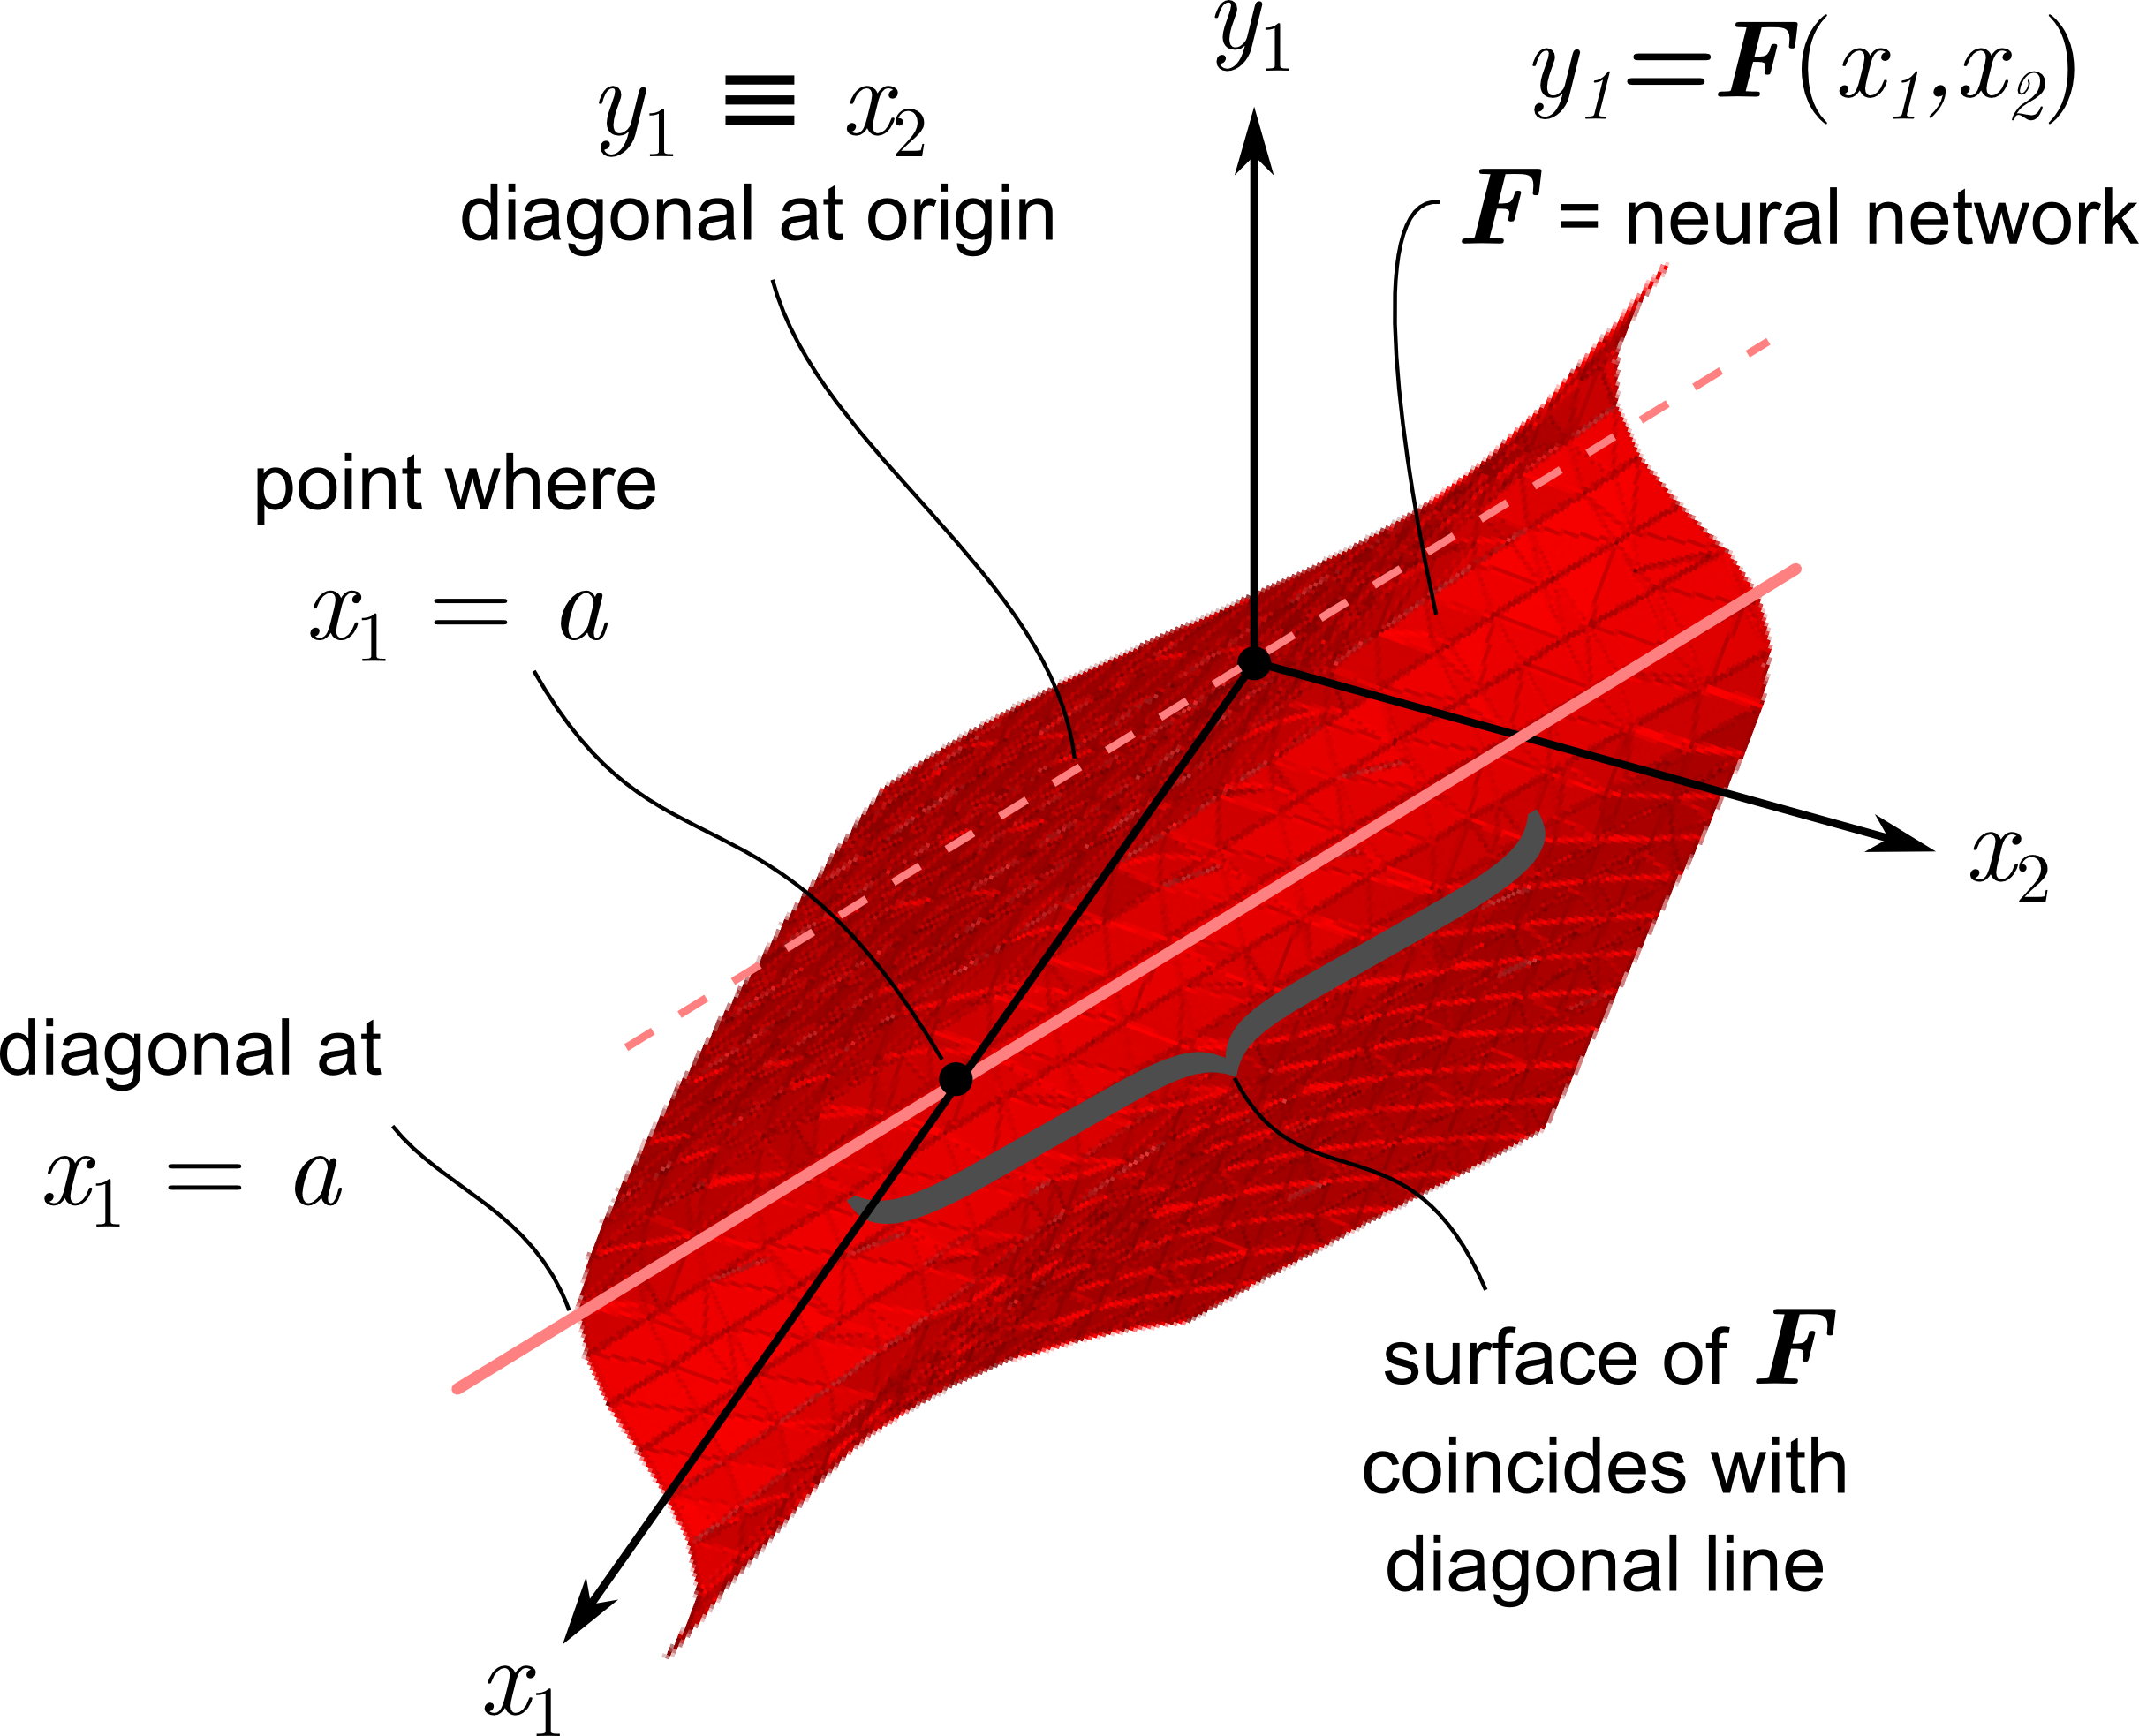
\includegraphics[scale=0.65]{linkage-geometric-view.png}
\label{fig:diagonals}
\end{equation}

\subsubsection{Learning algorithm with linkages}

As an optimization problem, the goal of learning is to find the optimal neural network $F^*$ in a function space (figuratively):
\begin{equation}
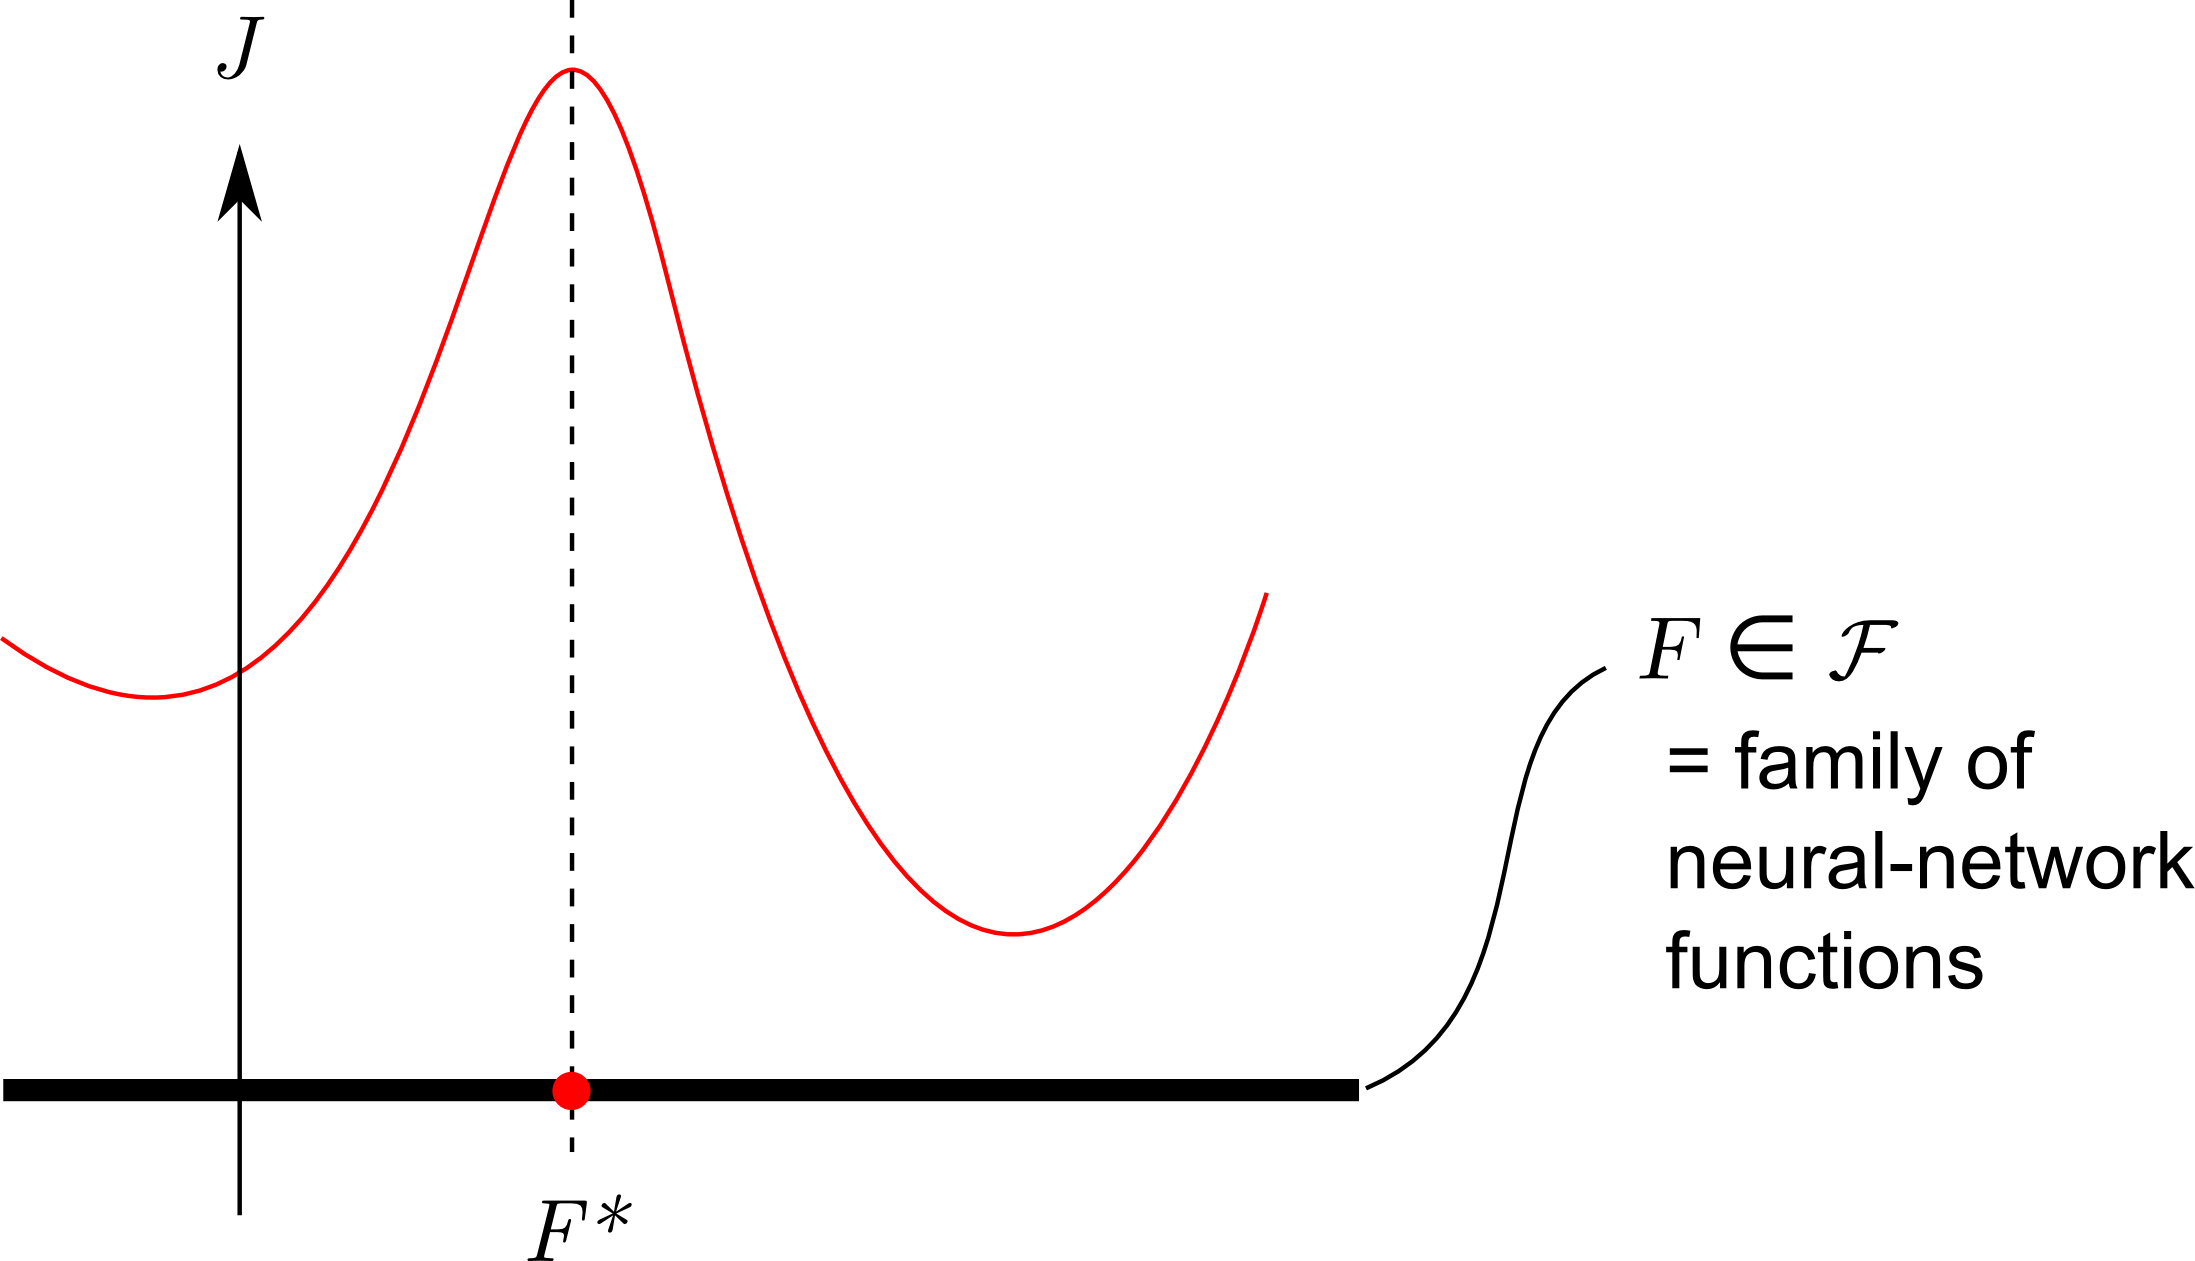
\includegraphics[scale=0.75]{gradient-descent.png}
\end{equation}
We need a new algorithm that gives priority (higher scores) to linkages:
\begin{equation}
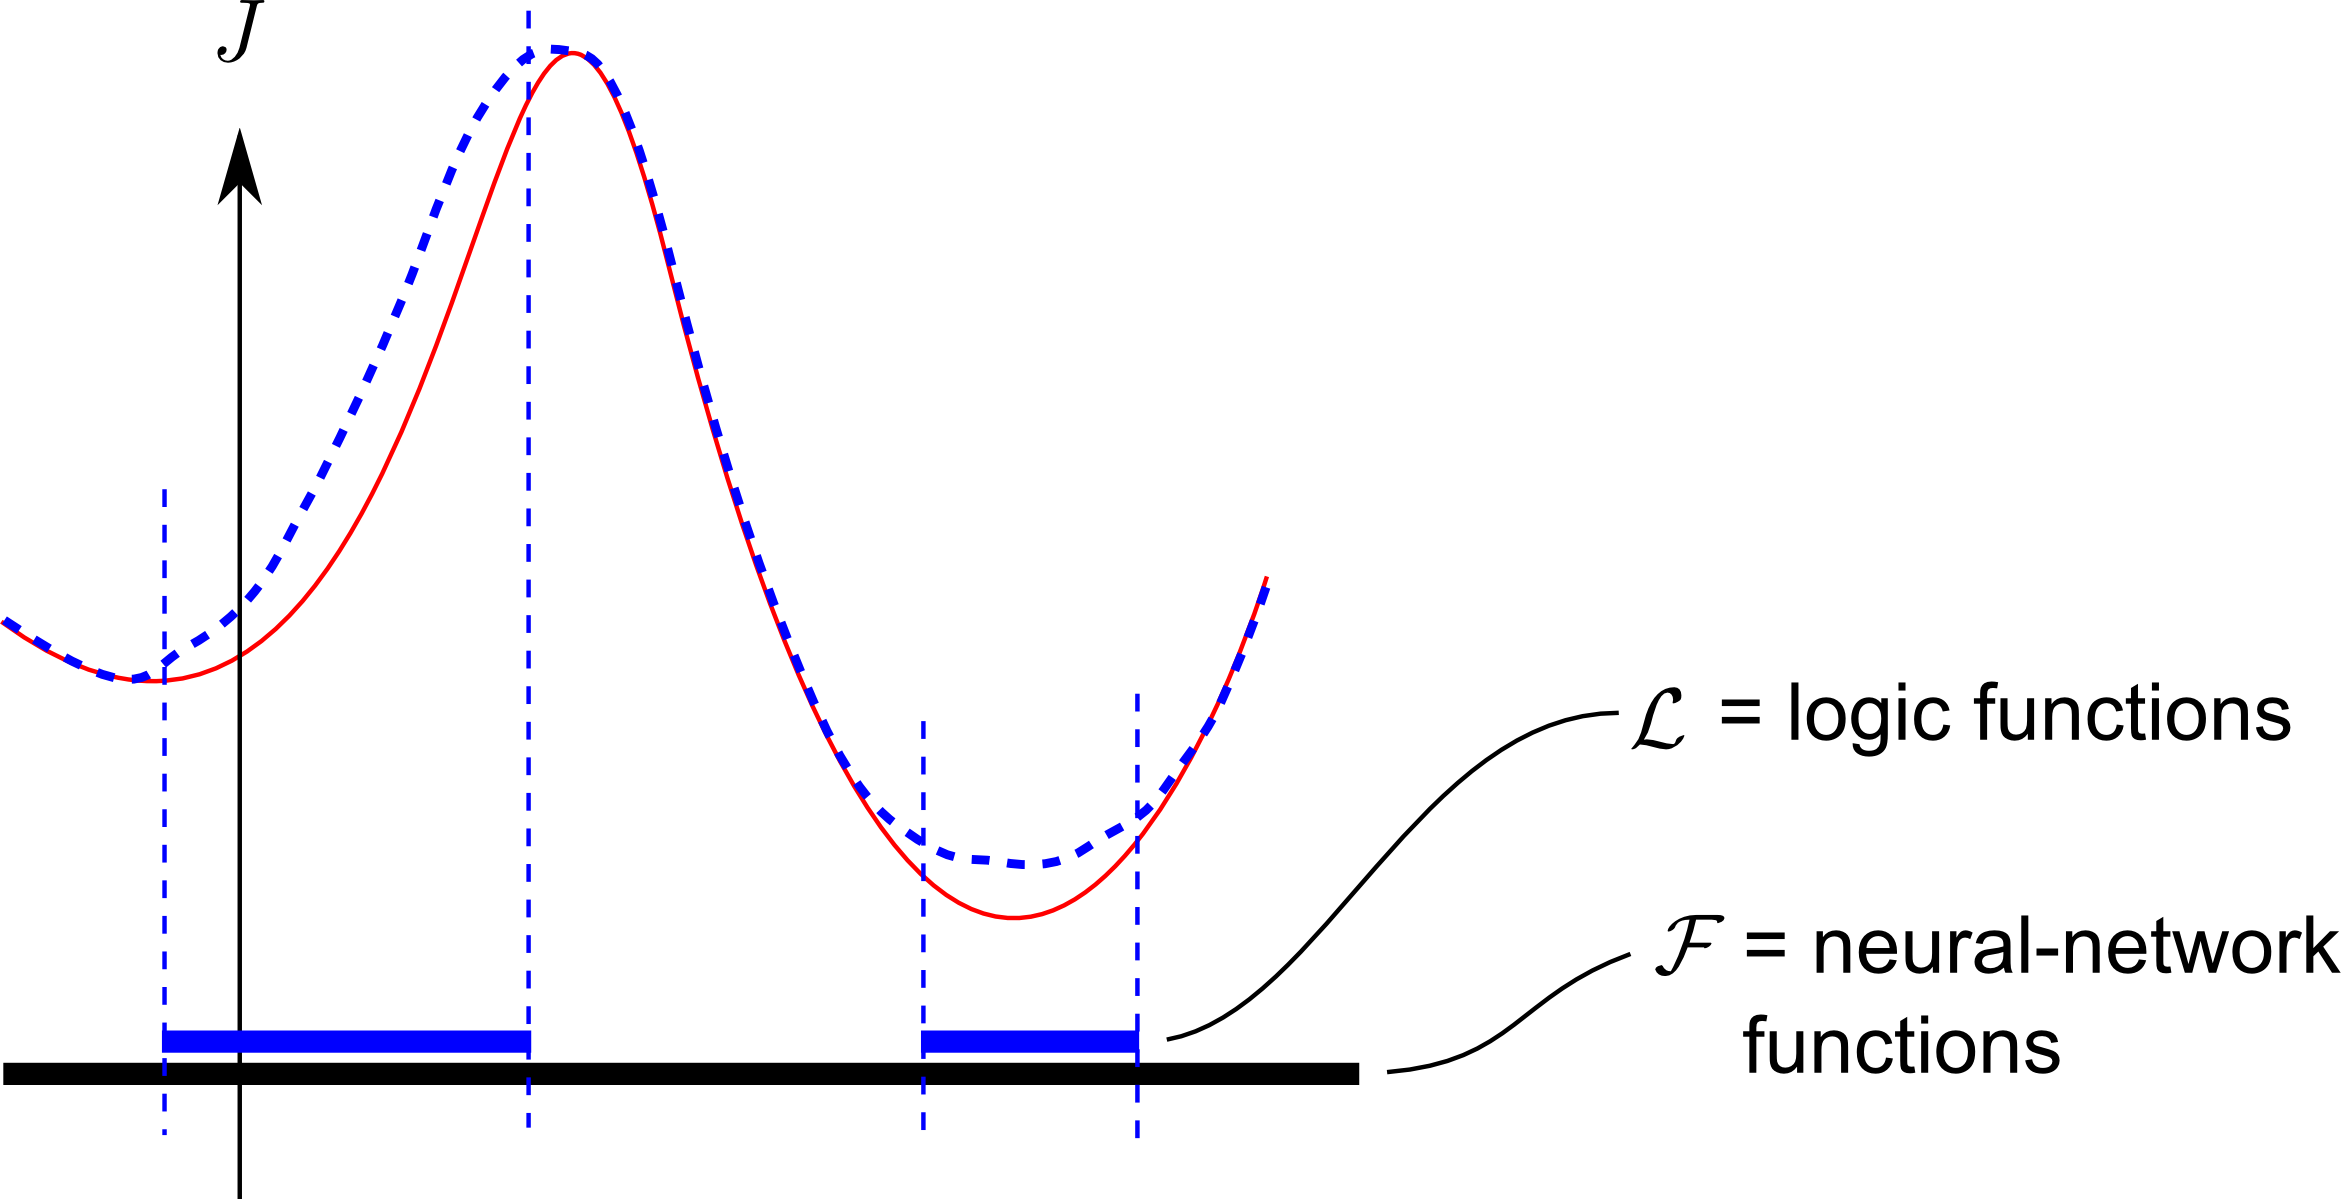
\includegraphics[scale=0.75]{gradient-descent-2.png}
\end{equation}

Below is a figure that shows the ``internal threads'' of a function ($\vdash$) that maps a premise to a conclusion, ie:
\begin{equation}
P_1 \wedge P_2 \wedge P_3 \wedge ... \quad \vdash \quad Q_1 \wedge Q_2 \wedge ...
\end{equation}
\begin{equation}
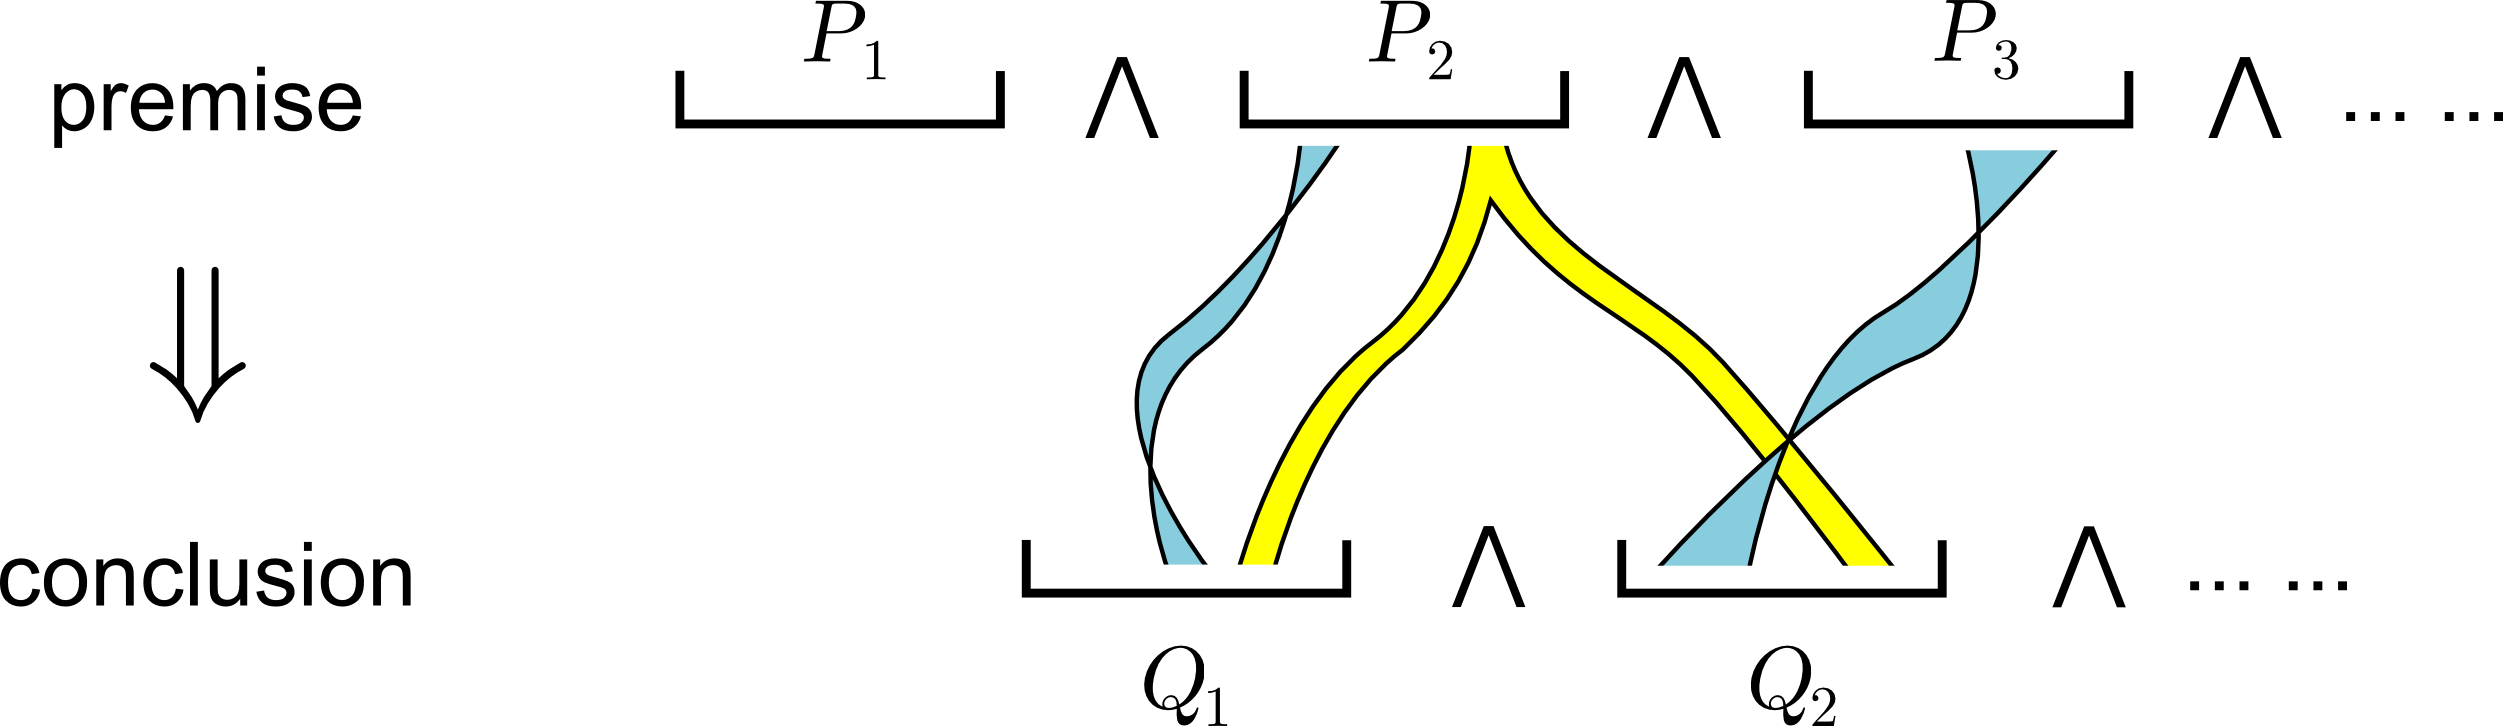
\includegraphics[scale=0.7]{linkage-propositional-view.png}
\end{equation}
where \colorbox{yellow}{yellow} ``ribbons'' represent $\mbox{id}$ mappings (that respect coordinate positions), \colorbox{cyan!20}{blue} ribbons represent abitrary mappings.

As for learning algorithm, one idea is to \textit{force} the learning of diagonals, whenever a potential identity function is detected.  This creates a ``propensity'' for generalization.  After a diagonal is learned, it may be destroyed by subsequent learning; which is fine.  Also, the forcing of a diagonal may accidentally destroy previously learned knowledge.  This may be balanced by \textbf{dual-lobe} re-normalization.
\newsavebox{\algbox}
\begin{lrbox}{\algbox}
\begin{minipage}{0.8\linewidth}
\begin{algorithm}[H]
 % \KwData{training data?}
 % \KwResult{learn linkages}
 % initialization\;
 \For{each data item}{
  detect if a potential identity may exist\;
  \eIf{identity seems to exist}{
   force-learn the diagonal\;
   }{
   learn as usual\;
  }
 }
 dual-lobe re-normalization\;
% \caption{How to write algorithms}
\end{algorithm}
\end{minipage}
\end{lrbox}
\begin{equation}
	\usebox{\algbox}
\end{equation}

\begin{tcolorbox}[breakable, enhanced]
\setlength{\parskip}{2.8ex}

\section*{Appendix: logic and logic-based AI}
\renewcommand{\thesection}{A}

This part is to be separated to become a tutorial paper...

\setcounter{subsection}{0}
\subsection{Algebraic logic}

Traditionally, there are 2 ways to express the \textbf{sub-propositional} structure of logic:  via \textbf{predicate logic} and \textbf{relation algebra}.  No matter which way, their essence is \textbf{variable substitution}.  Interestingly, substitution is also the essence of ``algebra'', but here substitutions occur \textbf{implicitly}, so it is actually difficult to use algebra to express them explicitly.

As for \textbf{$\lambda$-calculus}, it is essentially also a scheme for managing substitutions.  Whereas \textbf{combinatory logic}, equivalent to $\lambda$-calculus, eliminates the use of ``variables''.  The price to pay is an increase in length of the formulas (more complex than relation algebra).

The algebraization of (first-order) predicate logic is given by Alfred Tarski's \textbf{cylindric algebra}:
\begin{equation}
\frac{\mbox{propositional calculus}}{\mbox{Boolean algebra}} = \frac{\mbox{predicate calculus}}{\mbox{cylindric algebra}}
\end{equation}
The algebraization of \textbf{higher-order logic} (HOL) is provided by \textbf{topoi theory} \cite{Lambek1988} \cite{MacLane1992}:
\begin{equation}
\frac{\mbox{intuitionistic propositional calculus}}{\mbox{Heyting algebra}} = \frac{\mbox{higher-order logic}}{\mbox{elementary topos}}
\end{equation}
HOL is equivalent to \textbf{untyped} $\lambda$-calculus, whereas the \textbf{typed} $\lambda$-calculus (= type theory) is somewhat weaker.  The characteristic of the entire HOL family is ``substitution of equal by equals'', which causes the length of formulas to increase.  But predicate logic performs substitution with \textbf{objects}, so it does not increase the length of formulas;  However, its algebraization introduces notions such as cylindrification and the diagonal set.  For example, in fig. (\ref{fig:diagonals}) there is the diagonal $y_1 \equiv x_2$.

This is an illustration of \textbf{cylindrification}:
\begin{equation}
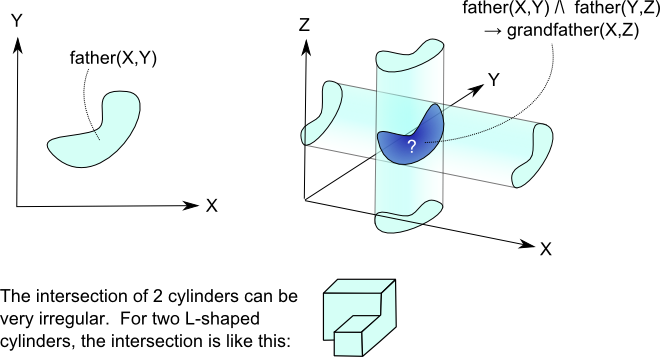
\includegraphics[scale=0.8]{cylindrification.png}
\end{equation}

\subsection{Relation algebra}

%Personally I think \textbf{relation algebra} \cite{Schmidt2010} \cite{Maddux2006} is closer to human natural language, but the standard form used in mathematical logic research is first-order logic (FOL).  This is however not of the essence, because all logics are basically easily interconvertable.  In the following we concentrate on FOL.
%个人认为 relation algebra \cite{Schmidt2010} \cite{Maddux2006} 比较接近人类自然语言,但在数理逻辑研究中最通用的逻辑是 first-order logic (FOL)。 然而这并不是重点,因为各种逻辑基本上是等效的,而且相互之间可以很容易地转换。 以下集中讨论 FOL。  

以前曾经对 relation algebra \cite{Schmidt2010} \cite{Maddux2006} 有些幢憬,因为它比较接近人类自然语言,但其实 relation algebra (RA) 和 first-order logic (FOL) 基本上是等效的,在 FOL 里面有 linkage 的复杂性,但在 RA 里面这个复杂性其实也没有消失。 可以说「\underline{复杂度是守恒的}」\footnote{这句话是 category theorist Eugenia Cheng 说的。}。

举例来说,在 (\ref{linkage-father}) 中表达「\textit{爸爸的爸爸是爷爷}」,可以用 RA 更简单地表达:
\begin{equation}
 \mbox{father} \circ \mbox{father} = \mbox{grandfather}
\end{equation}
实际的推导是这样的:
\begin{eqnarray}
\mbox{John father Pete} \nonumber \\
\mbox{Pete father Paul} \nonumber \\
\mbox{John father $\circ$ father Paul} 
\end{eqnarray}
这时要 \emp{代入} 上面的等式才能得出结论:
\begin{equation}
\mbox{John grandfather Paul}
\end{equation}
所以 linkage 的复杂性变成了代数 formula 长度的复杂性。 

\subsection{Fractal structure}

「长度」本身没有不妥,但我们的目的是将逻辑式子嵌入到状态空间 $\vect{x}$ 里,这时 variable length 令人很头痛,但 fixed length 没有此问题。 如果硬要将 variable length 的式子嵌入到(有限维)向量空间中,\uline{似乎必须用到 \emp{fractal} 结构}(因为它有自相似性),同时需要设计一种新的神经网络,它先天性地有 fractal 结构在里面; 但这比较复杂,我没有在这方向 explore。

\subsection{Trading space with time}

上面说的是 substitution 在空间中的 linkage 结构。 但也可以将 substitution \textbf{分拆}成若干个简单的步骤。 方法是: 将某些内容放进记忆体中的「盒子」中,\uline{这些盒子充当 variables 的角色,也就是很具体地实现 substitution 的动作}。 换句话说,将\textbf{空间复杂性}转换成\textbf{时间复习性}\footnote{人脑的脑电波由 0.5 Hz 到 40 Hz 都有,我们感觉上瞬间的动作可能已经过了若干次迴路。}; 以下是示意图:
\begin{equation}
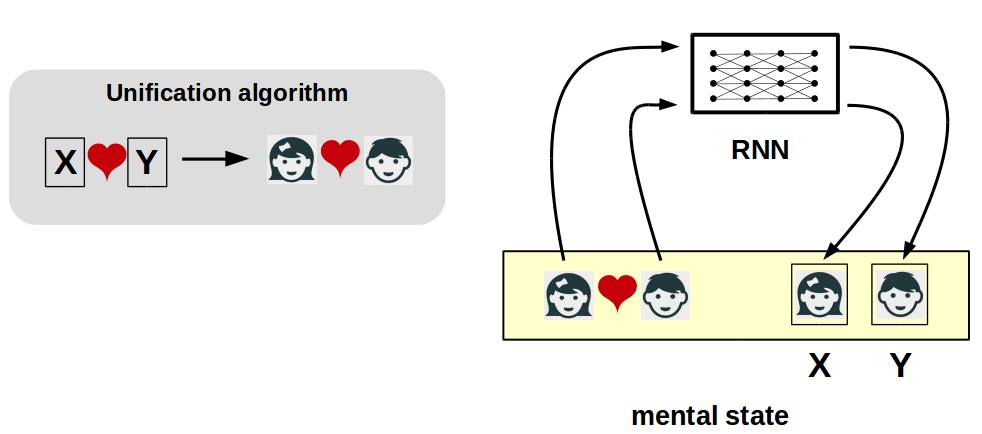
\includegraphics[scale=0.4]{unification-cartoon-2.jpg}
\end{equation}
X,Y 是状态空间 $\mathbb{X} \ni \vect{x}$ 里面的「盒子」 = variables。

先前我说的 linkage 结构,放在有限维向量空间比较方便,但它是 first-order logic,处理 higher-order 关系时有很大困难。 Higher-order relations 似乎还是要用这种分拆步骤的方法解决。

\subsection{Cartesian-closedness}

折腾了这么久,但仍然缺少了一个重要的特性: Cartesian-closedness。 它指的是在某个範畴内,对任意的 $A,B$,都必然可以找到它们的:
\begin{equation}
\boxed{\mbox{product}} \; A \times B \quad \mbox{和} \quad B^A \; \; \boxed{\mbox{exponentiation}} 
\end{equation}
In logic this refers to:
\begin{equation}
A \wedge B \quad \mbox{和} \quad A \rightarrow B
\end{equation}

为什么需要 Cartesian-closed?  注意在 minimal architecture 里,只有两种记忆,即瞬时记忆 $\vect{x}$ 和永久记忆 $\vect{F} = \KB \vdash$。 从 logic-based AI 的角度来看,$\KB$ 里装著 logic rules,但 $\vect{x}$ 里面只有 ground facts。 Ground sentence 指的是\textbf{没有变量}的命题,例如:
\begin{equation}
\vect{x} = \textit{见到地上有血迹}
\end{equation}
相比之下,logic rule 是有变量的 conditional statement,例如:
\begin{equation}
\forall Z. \quad \mbox{\textit{$Z$有血迹}} \rightarrow \mbox{\textit{$Z$可能是凶案现场}}
\end{equation}
如果在 $\vect{x}$ 里面可以存放 rule,那表示 $\vect{x} \ni \mathbb{X}$ 是一个 Cartesian-closed category。 这样的 $\mathbb{X}$ 是一个更 powerful 的结构,亦即系统可以思考更复杂的 thoughts。 更重要的是,$\vect{x} \ni \mathbb{X}$ 和 $F = \KB \vdash$ 现在\textbf{地位平等},因为它们都是 $\mathbb{X} \rightarrow \mathbb{X}$ 的\textbf{函数},因为 Cartesian-closed 表示 $\mathbb{X} \simeq \mathbb{X}^{\mathbb{X}}$。 这个特性在 belief revision 中似乎会很有用(见下节)。

如何在神经网络中做到 Cartesian-closed? 记得神经网络中 $\vect{x}$ 是一组 features $= (x_1, x_2, ..., x_n)$。 一个办法是将所有 $\vect{x}$ 都变成 $\mathbb{X} \rightarrow \mathbb{X}$ 的函数。 逻辑的 implication $A \rightarrow B$ 显然是函数,但单一 ground sentence $A$ 也可以是函数: $\top \rightarrow A$ ,其中 $\top$ 是逻辑「真」。 注意: 这些函数中可以有 linkages,即处理变量的能力。

转到神经网络中,$A \rightarrow B$ 是一个 $\mathbb{X} \rightarrow \mathbb{X}$ 的神经网络。 $\top \rightarrow A$ 也是一个 $\mathbb{X} \rightarrow \mathbb{X}$ 的神经网络,但它将 $\vect{1} \mapsto \vect{A}$。

那 $\mathbb{X}$ 是一个怎样的空间?  它本身可以是一个深度神经网路的 weights,但\uline{这个神经网络的输入/输出层必须有足够的}\textbf{\uline{阔度}}\uline{去处理}\textbf{\uline{它自己}}!  表面上似乎不可能.... 越多的 weights 需要更多的 weights 去处理.... 但如果令 $\vect{x}$ 储存一些 partial functions 或许可以。

\subsection{Application to belief revision}

Belief revision (也可以叫 ``truth maintenance'')是经典逻辑 AI 发展的高峰。 如果可以用我们的新 architecture 做到 belief revision,我们会很有信心这个理论是 general intelligence。 

正常的逻辑运作模式是由 $\KB$ 作用在 $\vect{x}$ 上给出新的 $\vect{x}$:
\begin{equation}
\KB ( \vect{x} ) = \vect{x}'
\end{equation}
但 belief revision 或者可以看成是 $\vect{x}$ 作用在 $\KB$ 上的结果:
\begin{equation}
\vect{x} ( \KB ) = \KB'
\end{equation}
由於 Cartesian-closedness,$\vect{x}$ 和 $\KB$ 的地位是平等的,使上面的运作成为可能。 

这只是一个 vague idea,我会再回到这里填补这空白....

\end{tcolorbox}

% ====================================================================================
\begin{comment}
\subsection{由一些命题推导出另一些命题}

命题也有内部结构(即命题可以由概念原子组合而成),但我们先从最简单情况谈起,即\textbf{命题逻辑}。

最简单的经典命题逻辑,是 Boolean propositional logic,它的\textbf{代数形式}是我们熟悉的 Boolean algebra,二者几乎没有分别(纯粹逻辑符号和代数符号的对应)。 

在 Boolean algebra 可以定义一种 ideal $I$:
\begin{itemize}
\item If $a, b \in I$ then $a \wedge b \in I$
\item If $a \in I$ and $a \le b$ then $b \in I$
\end{itemize}
其中 $a \le b$ 表示 $a \Rightarrow b$(a 蕴涵 b)。

由上面可以看出,这个 ideal 其实是由某些元素(命题)生成的 \textbf{逻辑后果}(logical consequence); 换句话说,给定一个命题集 $\Gamma$,问 $\Gamma \stackrel{?}{\vdash} a$(从 $\Gamma$ 可以推导出 $a$ 吗?) 就等於问 $a$ 是不是 $\Gamma$ 生成的 ideal membership 问题。 也可以说,代数 ideal $\equiv$ 逻辑 consequence。 (严格来说,consequence 对应的是 filter 的概念,而 filter 是 ideal 的 dual,因为 0 和 1 对应的倒错,但这不是重点。)

\textbf{逻辑后果}可以记作 $\vdash$ 或 Cn,Tarski 定义了 $\vdash$ (很明显)的特性:
\begin{itemize}
\item (reflexivity): \quad $A \vdash A$ for every formula $A$
\item (monotonicity): \quad $A \vdash Q$ implies $A, B \vdash Q$
\item (`cut'): \quad \quad $A \vdash B$ and $A, B \vdash Q$ implies $A \vdash Q$
\end{itemize}

% 在 Boolean algebra 中有一些 inference rules,例如:

以上是 Boolean logic 的代数化,但如果考虑 probabilistic logic 就更为复杂,需要用到 Bayesian networks,而 filter $\equiv$ consequence 的原理似乎不再适用。 

Bayesian network 的细节很麻烦,可以花整个研究生课程来讲。

重点是: Bayesian network 是由一些\textbf{条件概率} (conditional probability) 的关系生成的。 每个\textbf{节点}是一个命题,每个\textbf{连结}是一个条件概率关系,例如:
\begin{equation}
P(A|B,C,D,...) = \vec{p}
\end{equation}
其中 $\vec{p}$ 是一个 conditional probability table (CPT)。

对不起,用一个较粗俗的例子说明(在我多年的教学经验里,这是最易懂的例子):
\begin{equation}
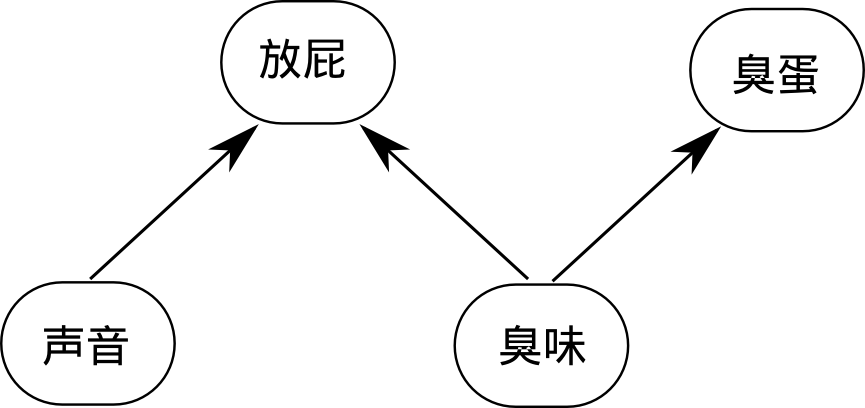
\includegraphics[scale=0.5]{farting.png}
\end{equation}
这个 Bayesian network 是由两个 CPT 生成的:
\begin{eqnarray}
P(\mbox{放屁} | \mbox{臭味}, \mbox{声音}) = \vec{p}_1 \nonumber \\
P(\mbox{臭蛋} | \mbox{臭味}) = \vec{p}_2
\end{eqnarray}
如果有「声音」又有「臭味」,则「有人放屁」的机率很高,而「臭蛋」的机率却会减少。 换句话说,「臭蛋」的机率被扯到「放屁」那边去了; 这个现象叫 ``explaining away'',它说明 Bayesian network 中,所有节点都是 globally 相关的。 所以,当求解 Bayesian network 的某个节点时,它的概率会是一连串很复杂的 sum-product 形式。 看来用 Bayesian network 表示 $\vdash$ 的方法太复杂了。

可幸的是,可以用 Monte Carlo 方法求解 Bayesian network: 开始时随机地指定节点的概率,然后随机地选取某些节点来作「\textbf{局部}」的 update; 当随机 update 的次数趋近无限,节点的机率会收敛到正确的值。 换句话说: 这是一个 \textit{local} 的计算 Bayesian network 的方法。

\section{Model theory}

For the basics of model theory, cf \cite{Doets1996} \cite{Manzano1999}.  The model-theoretic approach is to separate the \textbf{symbolic language} $\mathcal{L}$ and the $\mathcal{L}$-structures it refers to.  They are related by \textbf{interpretation} maps.

% 模型论基础可参看 \cite{Doets1996} \cite{Manzano1999}。 模型论的做法是将逻辑的符号\textbf{语言} (language $\mathcal{L}$) 和它所指涉的\textbf{结构} $\mathcal{L}$-structure 分割,中间用 interpretation map 关联起来。

$\mathcal{L}$ contains the set of symbols (predicates, relations, functions, constants), which recursively generates formulas and compound formulas.  These are the \textbf{symbolic} stuff.

%$\mathcal{L}$ 就是符号的集合 (predicates, relations, functions, constants),递归地生成出句子和复合句子。 这些都是 symbolic 的东西。

An $\mathcal{L}$-structure can be any abstract algebraic structure.  It usually consists of a \textbf{base set}, and functions and relations defined over that set.

%$\mathcal{L}$-structure 可以是任何抽象代数结构,它通常包含一个 base 集合,然后在集合上定义一些函数和关系。 

The central idea of model theory is using the interpretation map $i$ to ``preserve'' certain relations, for example:

%模型论的中心思想是透过 interpretation $i$ 去「保存」一些关系,例如:
\begin{equation}
R(a,b) \stackrel{i}{\mapsto} R^\mathcal{M}(a^\mathcal{M}, b^\mathcal{M})
\end{equation}

$R$ is a relation, $x^\mathcal{M}$ denotes the object corresponding to $x$ in the structure $\mathcal{M}$.  The left side is symbolic logic;  the right side is the actual structure.  When model theory is applied to first-order logic, we get the equivalence of $\vdash$ and $\vDash$ (which looks like tautology).  This can be found in any mathematical logic textbook, such as \cite{Hedman2004}.

%$R$ 是一个关系,$x^\mathcal{M}$ 代表在结构 $\mathcal{M}$ 之上,$x$ 所对应的物体。 左边是符号逻辑,右边是实体的结构。 模型论应用在 first-order logic,得出 $\vdash$ 和 $\vDash$ 等价的结论(看起来就好像同语反覆),这在数理逻辑教科书中都有,例如 \cite{Hedman2004}。 

If we use category theory to express the correspondence between logic and neural:
%如果用範畴论的方法表示逻辑结构和神经结构之间的对应:
\begin{equation}
\begin{tikzcd}[]
\mathcal{L} \arrow[d, "i"] \\
\mathcal{M} \arrow[r, phantom, "\simeq"] & \mathcal{X} \\
& \arrow[u, "\mbox{deep NN}" swap] \mathcal{S}
\end{tikzcd}
\end{equation}
\begin{itemize}
\item $\mathcal{L}$ = category of logic theories (= sets of formulas)
\item $i$ = interpretation maps
\item $\mathcal{M}$ = category of models (from logic)
\item $\mathcal{X}$ = category of models (from deep NNs)
\item $\mathcal{S}$ = sensory input
\end{itemize}

The above diagram says the same as this cartoon explanation:
%上图等同於下面的卡通解释:
\begin{equation}
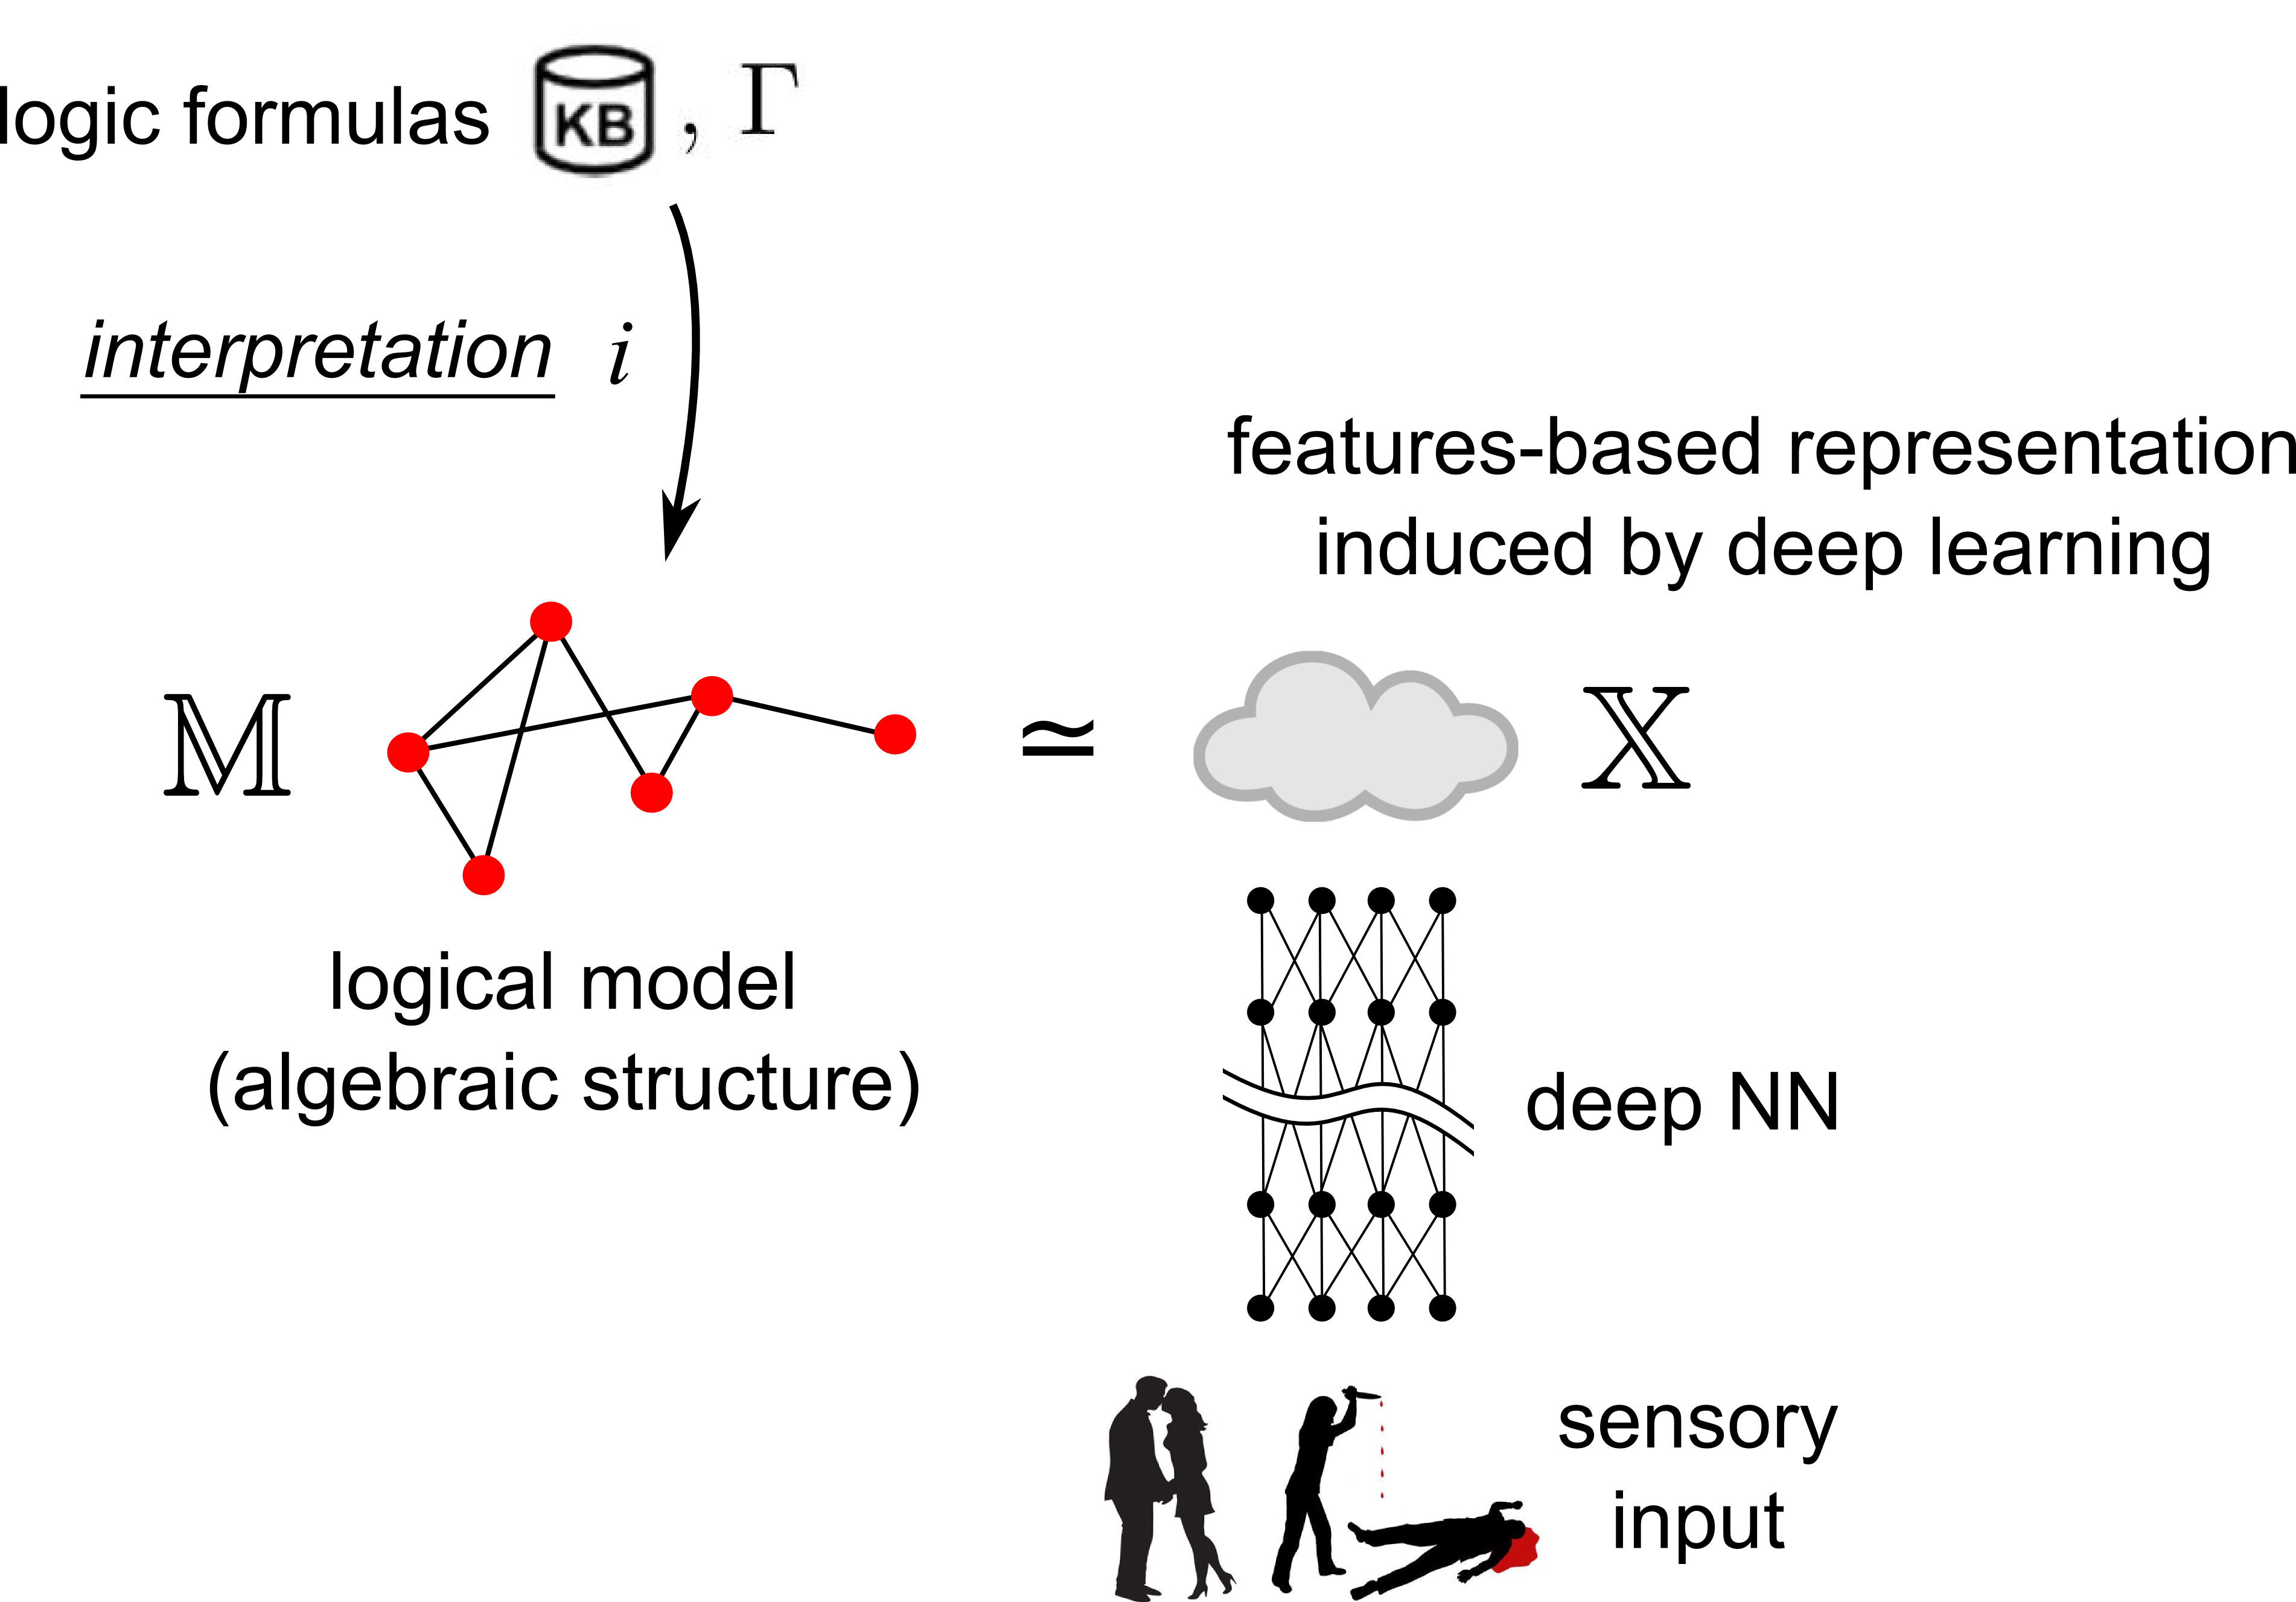
\includegraphics[scale=0.7]{model-theory-cartoon.png}
\end{equation}

In other words, $\mathcal{X} = \vcenter{\hbox{
\includegraphics{cloud.png}}}$ is \textbf{induced} from deep learning;  but its structure is \textbf{opaque} to us (that is the weakness of neural networks).
%换句话说,$\mathcal{X} = \vcenter{\hbox{
\includegraphics{cloud.png}}}$ 是由深度学习 induce 出来的结构; 但它的结构对我们来说是不透明的(这是神经网络的弱点)。

Whereas, the structure of $\mathcal{M} = \vcenter{\hbox{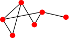
\includegraphics{algebraic-model.png}}}$ is the subject matter of model theory.

%而 $\mathcal{M} = \vcenter{\hbox{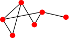
\includegraphics{algebraic-model.png}}}$ 的结构就是模型论研究的对象。
%是 free 的; 换句话说,那 $i$ map 的 source domain 是固定的,但 target domain 是自由的。 这导致 $i$ map 的学习很困难,因为 $\mathcal{M}$ 和 $\mathcal{X}$ 的结构都不清楚。 必须更详细分析 $\mathcal{M}, \mathcal{X}$ 的结构。

\section{模型论和 interpretation 的结构}

In model theory, $\mathcal{L}$ is the category of logic formulas, $\mathcal{M} = \vcenter{\hbox{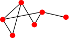
\includegraphics{algebraic-model.png}}}$ could be any algebraic structure.  We just need to map the constants, predicates, relations, functions in $\mathcal{L}$ to the structure in $\mathcal{M}$.  For the sake of conciseness, we will just constants symbols and relation symbols, as these two are the \textbf{essence} of logic.

%在模型论中,$\mathcal{L}$ 是逻辑句子的範畴,$\mathcal{M} = \vcenter{\hbox{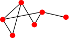
\includegraphics{algebraic-model.png}}}$ 可以是任何抽象代数结构。 只需把 $\mathcal{L}$ 中的 constants, predicates, relations, functions 映射到 $\mathcal{M}$ 就行。 为简化讨论,我们只考虑 constants 和 relations,因为二者是逻辑中最\textbf{本质}的东西。 
\begin{eqnarray}
\mathcal{L} & \quad \stackrel{i}{\rightarrow} \quad & \mathcal{M} \nonumber \\
\mbox{constant symbol} & \quad \stackrel{i}{\mapsto} \quad & \; 
\includegraphics[scale=0.5]{node.png} \\
\mbox{relation symbol} & \quad \stackrel{i}{\mapsto} \quad & \; 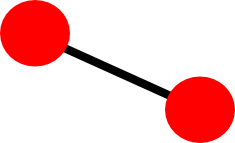
\includegraphics[scale=0.5]{link.png} \nonumber
\end{eqnarray}

Our problem is that we don't know the structure of  $\vcenter{\hbox{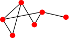
\includegraphics{algebraic-model.png}}}$.  For a long time, researchers have treated neural networks as ``black boxes'', but if we don't know the structure of $\mathcal{X} =  \vcenter{\hbox{
\includegraphics{cloud.png}}}$ we cannot build the isomorphism $\mathcal{M} \simeq \mathcal{X}$.

%问题是在神经那边缺乏 $\vcenter{\hbox{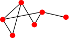
\includegraphics{algebraic-model.png}}}$ 的结构。 一直以来,人们习惯把神经网络看成是 ``black box'',但如果我们不知道 $\mathcal{X} =  \vcenter{\hbox{
\includegraphics{cloud.png}}}$ 的结构,就无法建立 $\mathcal{M} \simeq \mathcal{X}$ 的 isomorphism。

\section{Conclusion}

This paper is not very successful because we have jumped to the conclusion  (\ref{conclusion1}) and (\ref{conclusion2}) without rigorous justification:  They are merely intuitively plausible.  In theory, since we have known how $\mathcal{M}$ is generated, and how $\mathcal{X}$ is generated, it should be feasible to build a ``highway'' between them.  In practice, it seems that we just need a deep neural network, because neural networks are \textbf{universal function approximators}, we don't even need to care about the structure between $\mathcal{M}$ and $\mathcal{X}$.

%这篇论文并不太成功,因为跳到 (\ref{conclusion1}) 和 (\ref{conclusion2}) 的结论没有严谨的根据,只是直观上觉得有可能。 理论上来说,既然知道了 $\mathcal{M}$ 那边是怎样生成的、$\mathcal{X}$ 那边是怎样生成的,则要在两边建立「高速公路」应该是可行的。 实际上,似乎只要建立一个深度网络就可以,因为神经网路是 universal function approximator,根本不用考虑 $\mathcal{M}$ 和 $\mathcal{X}$ 这两个结构之间的关系。

For further research, I hope some professional mathematicians can help with these problems:
%进一步的研究,希望数学专业的人能帮助一下:
\begin{enumerate}
\item On the logic side, could we transform its structure to one in \textbf{algebraic geometry}? In other words:  logic formulas $\simeq$ algebraic equations.  I only know of one instance of this kind of algebraic logic: Andreka \textit{et al}'s \cite{Andreka2001}, it seems to be an esoteric research area.
%\item 在逻辑那边,可不可以转换成 algebraic geometry 的结构? 即是说: 逻辑式子 $\simeq$ 代数方程。 这种代数逻辑的做法,我暂时只知道有 \cite{Andreka2001},是很偏门的研究。
\item From the structure of $\mathcal{M}$ and $\mathcal{X}$, can we find out the simplest form of a bridge between them?  Perhaps using mathematical induction, we examine the generative process of $\mathcal{M}$ and $\mathcal{X}$ layer by layer?
%\item 能不能根据 $\mathcal{M}$ 和 $\mathcal{X}$ 的结构,找出它们之间的桥的最简单形式?  可以用数学归纳法,逐步考虑 $\mathcal{M}$ 和 $\mathcal{X}$ 生成的方式,或许有帮助?
\end{enumerate}

%看上去颇复杂,但这样已经可以直接由逻辑式子 $\mathcal{L}$ 映射到深度网络的输出层。  在未有这理论之前,完全不知道这个 map 的结构;  但现在假如理论是正确的话,只需要简单的组合搜索 (combinatorial search) 就可以找到对应。  

\textbf{Application}:  When applying deep learning to natural language understanding, this theory may be helpful.
%应用: 对於用深度学习做 natural language understanding 的人,这理论或许会很有用。 

% Armed with this theory, we may construct an actual neuro-logic bridge.

\section{Prior art}

\begin{itemize}
\renewcommand\labelitemi{\textbullet}

\interfootnotelinepenalty=10000

\item Bader, Hitzler, H\"{o}lldobler and Witzel proposed in 2007 a method of neural-symbolic integration \cite{Bader2007}.  First they generate a Herbrand model\footnote{Herbrand model is a common construct in logic-based AI.  The gist is to generate from the logic language $\mathcal{L}$ ``whatever that can be instantiated'', resulting in an (often infinite) set of ground sentences (ie, without variables).  In other words, Herbrand models are generated from the language $\mathcal{L}$ self-reflexively, without relying on any external structure.  Every logic theory has at least one Herbrand model.} from the logic theory, maps the Herbrand model to a fractal space, and then directly use a neural network to learn that fractal space.  Though they used model theory, they did not make use of the correspondence between $\mathcal{M}$ and $\mathcal{X}$ in this paper.

%\item Bader, Hitzler, H\"{o}lldobler and Witzel 在 2007 年提出了一个 neural-symbolic integration 的做法 \cite{Bader2007}。 他们首先由 logic theory 生成抽象的 Herbrand model\footnote{Herbrand model 是邏輯 AI 中常用的概念,大意是用邏輯語言 $\mathcal{L}$ 生成「所有可以代入的東西」(instantiating whatever that can be instantiated),由此產生的不含變量的句子 (sentence) 的集合。 換句話說,Herbrand model 的特點是它只靠 $\mathcal{L}$ 自身產生它的模型,而不依賴任何外在結構。 每个邏輯 theory 都必然至少有一个 Herbrand model。},再将 Herbrand model 映射到某个 fractal 空间,然后直接用神经网络学习那 fractal 空间。  虽然用了 model theory,但他们没有利用到本文所说的 $\mathcal{M}$ 和 $\mathcal{X}$ 之间的关系。 

\item Khrennikov, in a series of papers starting from 1997, proposed using $p$-adic algebra to model the mental space $\mathcal{X}$, see his book co-authored with Anashin \cite{Anashin2009}.  A $p$-adic number can be regarded as a ``decimal'' number in base $p$, where $p$ is any prime.

\item Classical logic is binary;  There has been countless attempts to extend it to fuzzy or probablistic logic (eg. I have attempted in \cite{Yan2012}), but there is still not a unified concensus theory.  A slightly different approach, is to regard points in a space as first-order objects, and predicates as functions over that space.  Then we get a metric structure and on it a continuous first-order logic (CFOL) ~ \cite{Yaacov2008}.  This is a possible structure for $\mathcal{M}$.
%\item 经典逻辑是二元逻辑,近代已经有无数将它扩充到 fuzzy 或 probablistic 的尝试(作者也提出过 \cite{Yan2012}),但仍未有统一的理论。 与此不同的另一个方向,如果将点看成是 first-order objects,谓词是点空间上的函数,直接得到 metric structures 上的连续逻辑 (continuous first-order logic) ~ \cite{Yaacov2008},这可以看成是一种 $\mathcal{M}$ 的结构。

\item In model theory there  are ultra-filters and ultra-products, which originated in functional analysis.  Recently there has been novel research crossing between model theory and Banach space \cite{Iovino2002}.  Simply put, the ultra-product is a way to multiply existing models to yield new models.  I looked at it briefly and found that ultra-products often involve sets of infinite cardinality and are very ``big'' constructs.  So they may not be very practical for computational implementation.

\end{itemize}

% ==================================================================================
\end{comment}

\section*{Acknowledgement}

\footnotesize{Thanks to Ben Goertzel for discussions on the AGI mailing list.  Ben first pointed out the advantage of neural network learning over inductive logic learning, which prompted me to research their relationships.  Thanks also to Juan Carlos Pinto for personal discussions on the structure of neural networks.}

% =====================================================================================
\begin{comment}
\section{逻辑变量的处理}

这可能是最辣手的部分。

Alfred Tarski 提出了 cylindrical algebra 来解决「一阶谓词逻辑」的变量问题,但据说 Tarski 自己也觉得 cylindrical algebra 「不好用」。 我觉得它比较难明,从略。

个人觉得比较好的做法是 Paul Halmos 的 algebraic logic。 其中最关键的建构是:
\renewcommand\labelitemi{--}
\begin{eqnarray}
\mbox{谓词} : \mbox{物体} & \rightarrow & \mbox{命题空间} \nonumber \\
\cancel\heartsuit : \cancel\heartsuit(\mbox{john}) & \mapsto & \mbox{「阿 John 失恋」} \nonumber \\
\cancel\heartsuit : \cancel\heartsuit(\mbox{pete}) & \mapsto & \mbox{「阿 Pete 失恋」}
\end{eqnarray}
换句话说,predicate(谓词)就是一些将 object (逻辑中的物体,或「常项」,constants)映射到个别命题的\textbf{函数}。 这些谓词函数可以有一个或多个\textbf{参数},分别叫 monadic 和 polyadic predicate calculus。

最新的逻辑代数化方法来自\textbf{範畴论},William Lawvere 在 1960's 年代提出(也就是 \textit{Conceptual Mathematics} 这本书的作者之一)。  他发现了 $\forall$ 和 $\exists$ 是 adjoint functors 的关系; 这个 adjunction 比较难懂,有兴趣可以看 \cite{Lawvere2003}。
\end{comment}
% =====================================================================================

\bibliographystyle{plain} % or number or aaai ...
\bibliography{AGI-book}

\end{document}